\documentclass{tropLaClasse}
\usepackage{lipsum}
\usepackage{float}

%----------- Informations du rapport ---------

% Le type de rapport
\typestage{Rapport de stage de M1}

% Le lieu du stage
\institut{Institute of Science Tokyo}
\laboratoire{Nakashima Laboratory}

% Le VRAI titre de ton stage
\titre{Étude sur la commande de mouvement et contrôle du robot humanoïde nageur SWUMANOID} 

% Tes informations
\eleve{Clément MESPOUILLES}
\mention{Master Sciences de l'ingénieur -- Sorbonne Université}
\filiere{Parcours ROBOT}
\master{N° Étudiant : 21207226}
\trigrammemention{CMI Mécanique}

% Dates
\dates{01/06/2026 -- 31/08/2026}

% Les encadrants et l'année
\annee{2025/2026}
\tuteurentreprise{
    Motomu NAKASHIMA\\
    Daito NAGATA\\
    Hiroki YANADORI
}

%----------- Initialisation -------------------
\logoentreprise{logos/logo_tokyo.png} 

\begin{document}

\fairemarges
\fairepagedegarde

% ==========================================
%                 RÉSUMÉ
% ==========================================
\clearpage
\pagestyle{empty} % Pas de numéro de page pour le résumé
\section*{Résumé}
\textit{Cette page est dédiée au résumé du stage. A compléter à la toute fin. Elle doit généralement présenter le contexte, les objectifs, les méthodes utilisées et les principaux résultats.}

% ==========================================
%           TABLE DES MATIÈRES
% ==========================================
\clearpage
\setcounter{page}{1}
\pagestyle{plain} % On remet la numérotation des pages
\tabledematieres  % Commande déjà présente dans ton fichier .cls !

% ==========================================
%           CORPS DU RAPPORT
% ==========================================
\section{Introduction}
Ceci est le début de mon rapport. Je peux citer des articles scientifiques très facilement comme ceci : \cite{nakashima_2024}.

\subsection{Contexte du laboratoire Nakashima}
\lipsum[1]

\subsection{Le projet SWUMANOID}

\lipsum[1]

\newpage

\subsection{Missions assignées}

Le projet SWUMANOID vise à développer le firmware d'un contrôleur de robot humanoïde. Le système embarqué est construit sur le système de compilation \textbf{PlatformIO}, utilisant le framework \textbf{Arduino} sur un microcontrôleur \textbf{Espressif ESP32-S3}. Le firmware gère le contrôle en temps réel des servomoteurs via un bus RS-485 Dynamixel, la mesure inertielle, la communication sans fil via un point d'accès Wi-Fi, et la lecture de mouvements à partir de fichiers stockés sur le système de fichiers flash interne.

L'architecture logicielle est organisée autour d'une machine à états finis (\texttt{AppState} : \texttt{Boot}, \texttt{Idle}, \texttt{Loading}, \texttt{Ready}, \texttt{Running}, \texttt{Stopping}, \texttt{Error}), pilotée par des commandes UDP reçues depuis une interface web. Les données des capteurs, la télémétrie des moteurs et l'état du système sont périodiquement diffusés en retour au client.

Le firmware d'origine a été écrit et validé pour la carte de développement \textbf{M5Stack AtomS3}. À mon arrivée au laboratoire, le matériel avait été mis à niveau vers le \textbf{M5Stack AtomS3R}. Bien que les deux cartes partagent le même SoC ESP32-S3 et un facteur de forme similaire, elles diffèrent par deux composants matériels qui affectent directement le firmware :

\begin{table}[h!]
\centering
\begin{tabular}{lll}
\toprule
\textbf{Composant} & \textbf{AtomS3} & \textbf{AtomS3R} \\
\midrule
Capteur IMU        & MPU6886 (I2C 0x68) & BMI270 \\
Rétroéclairage de l'écran & GPIO direct        & Pilote LED I2C\\
\bottomrule
\end{tabular}
\caption{Différences matérielles entre l'AtomS3 et l'AtomS3R}
\end{table}

Le système précédent du SWUMANOID présentait plusieurs limites : une fréquence de contrôle bloquée à 72 Hz, des instabilités de communication sans fil (Wi-Fi/BLE), et une gestion fastidieuse des cartes SD pour les logs. L'objectif global de mon travail est d'améliorer drastiquement les performances et la stabilité du robot.

Pour cela, le \textbf{M5Stack AtomS3R} (intégrant un ESP32-S3) est beaucoup plus performant que son prédécesseur en raison de sa puissance (dual-core) et de sa RAM intégrée (PSRAM). Cela nous permet de :
\begin{itemize}
    \item Atteindre une boucle de contrôle très rapide à \textbf{200 Hz} pour 21 moteurs, offrant des mouvements fluides et réactifs.
    \item Gérer le Wi-Fi sur un cœur du processeur pendant que le second cœur gère exclusivement les moteurs de manière déterministe (sans être interrompu par le réseau).
    \item Remplacer la lenteur des cartes SD par une écriture ultra-rapide des logs directement dans la PSRAM du microcontrôleur.
\end{itemize}


Ma première mission technique consistait à \textbf{migrer la couche des pilotes matériels} d'un accès aux registres codé à la main et spécifique à la carte, vers la bibliothèque d'abstraction \textbf{M5Unified}, qui prend en charge nativement à la fois l'AtomS3 et l'AtomS3R. La migration a été circonscrite à deux pilotes, en préservant entièrement le reste de l'architecture du firmware :

\begin{enumerate}
  \item \textbf{\texttt{src/firmware/drivers/imu\_driver.cpp}}:remplacer l'accès brut aux
        registres I2C (spécifique au MPU6886) par des appels \texttt{M5.Imu}.
  \item \textbf{\texttt{src/firmware/drivers/display\_driver.cpp}}: s'assurer que l'écran LCD
        et son contrôleur de rétroéclairage sont correctement initialisés via M5Unified sur
        l'AtomS3R.
\end{enumerate}

La contrainte était explicite : \textit{ne pas modifier la logique globale de la machine à états}. Seule la couche matérielle devait être adaptée.

\section{Création d'une interface Web pour le contrôle}
Plutôt que de lancer tout le code complexe d'un coup, j'ai procédé méthodiquement en validant chaque brique technologique.

\subsection{Migration du Code et prise en main}
Le code d'origine était conçu pour l'AtomS3. Bien que l'AtomS3R soit similaire visuellement, son architecture interne est très différente. J'ai dû réécrire une partie des pilotes (drivers) matériels :
\begin{itemize}
    \item \textbf{L'écran LCD :} Sur l'AtomS3, le rétroéclairage était contrôlé directement par une broche (GPIO). Sur le S3R, il faut communiquer en I2C avec une puce dédiée (AW9523).
    \item \textbf{L'IMU (Centrale inertielle) :} Le capteur est passé d'un MPU6886 à un capteur de nouvelle génération. J'ai dû adapter le code pour lire correctement les nouvelles adresses I2C.
\end{itemize}

Puisque le cahier des charges souligne que le Wi-Fi est souvent instable, je ne pouvais pas me contenter de suppositions. J'ai implémenté un système de diagnostic réseau :
\begin{itemize}
    \item J'ai modifié le firmware pour qu'il calcule le \textbf{RSSI} (Received Signal Strength Indicator), c'est-à-dire la puissance réelle du signal Wi-Fi perçu par le robot.
    \item J'ai créé une interface web de contrôle avec un \textbf{graphique en temps réel (via Chart.js)} qui trace l'évolution de ce signal. Cela nous permet de localiser les zones de perte de paquets et de valider scientifiquement la qualité de la connexion avant de lancer le robot dans l'eau.
\end{itemize}


\subsection{Nouvelle Architecture Web}
L'objectif principal de cette deuxième phase de développement était d'intégrer directement sur l'UI utilisateur, l'interface qui permet de gérer le micro contrôleur, toutes les fonctionnalités pour pouvoir contrôler le SWUMANOID correctement et facilement en intégrant la possibilité d'upload des fichiers de mouvement directement issus de SWAM (.dat) et convertis directement lors de l'upload du fichier afin de créer une interface de contrôle web autonome, fluide et sécurisée. La logique de conversion des trajectoires a été intégralement déportée côté client (JavaScript), la méthode de conversion a été réalisée en reprenant le code MATLAB utilisé précédemment et donné par Iroki-san.\\

Plus précisément, lors du parsing du fichier \texttt{.dat} en JavaScript, chaque angle articulaire est converti en ticks Dynamixel selon la formule affine des moteurs série X :
\begin{equation}
tick = \frac{\theta_{deg}+180}{360} \times 4095
\end{equation}
Cette conversion intègre un arrondi entier et un clamp dans l'intervalle $[0, 4095]$.\\

L'AtomS3R agit désormais comme un simple exécuteur : il reçoit la trajectoire sous forme d'un unique bloc binaire compact, ce qui l'immunise contre les instabilités du réseau Wi-Fi lors de la lecture. Ce format binaire (little-endian) minimise drastiquement la taille du transfert réseau. La structure de ce paquet est détaillée dans le tableau \ref{tab:binary_payload}.

\begin{table}[h]
\centering
\begin{tabular}{|c|c|l|}
\hline
\textbf{Offset} & \textbf{Type} & \textbf{Contenu} \\ \hline
0 & \texttt{uint8} & Version ($=1$) \\ \hline
1 & \texttt{uint8} & Nombre de moteurs $N$ \\ \hline
2-5 & \texttt{uint32} & Nombre de frames $F$ \\ \hline
6 à $5+N$ & $N \times \texttt{uint8}$ & IDs des moteurs (ordre des colonnes) \\ \hline
$6+N$ à fin & $F \times N \times \texttt{uint16}$ & Ticks (row-major) \\ \hline
\end{tabular}
\caption{Structure du paquet binaire de la trajectoire transmis via l'API}
\label{tab:binary_payload}
\end{table}

La taille totale de la charge utile (en octets), notée $S$, dépend directement du nombre de moteurs $N$ et du nombre de frames $F$. D'après la structure détaillée dans le tableau \ref{tab:binary_payload}, la formule générique se décompose ainsi :
\begin{equation}
S(N, F) = 6 + N + 2NF
\end{equation}
Où $6$ octets correspondent à l'en-tête fixe (Version, Nombre de moteurs, Nombre de frames), $N$ octets représentent le tableau des identifiants moteurs, et $2NF$ octets contiennent les données de trajectoire brutes (chaque position étant codée sur un entier non signé de 16 bits, soit 2 octets).\\

Dans notre configuration, le SWUMANOID est actionné par $N = 21$ moteurs. Pour l'envoi d'une trajectoire comprenant $F = 144$ frames, le calcul exact de la taille du transfert réseau est le suivant :
\begin{align*}
S(21, 144) &= 6 + 21 + 2 \times 21 \times 144 \\
S(21, 144) &= 27 + 2 \times 3024 \\
S(21, 144) &= 27 + 6048 \\
S(21, 144) &= 6075 \text{ octets}
\end{align*}

Avec un \textit{payload} réseau strictement égal à 6075 octets (environ 6,07 kB), l'AtomS3R peut aisément absorber la totalité de la trajectoire en un seul envoi. L'interface web a été repensée en cinq panneaux verticaux (Status, Network \& Scan, IMU Lab, Motion Control, Motion Settings \& Logs) pour une meilleure lisibilité. Enfin, les communications temps réel reposent désormais sur des \textit{Server-Sent Events} (SSE) unidirectionnels plutôt que sur des WebSockets, éliminant ainsi les problèmes de gigue (\textit{jitter}) et de collision sur le bus RS-485.


\subsection{Implémentation de la Télémétrie et Gestion Mémoire}

\paragraph{Résilience réseau :}
Dans le contexte d'une utilisation sous-marine, les micro-coupures Wi-Fi figeaient fréquemment l'interface web sans en avertir l'utilisateur. Pour rendre le système résilient aux pertes de signal, j'ai développé un \textit{Watchdog} en JavaScript qui surveille le flux \textit{Server-Sent Events} (SSE). S'il n'y a pas de données reçues pendant 600 ms, l'interface affiche une alerte \og OFFLINE \fg{} et tente une reconnexion silencieuse.

\paragraph{Le défi de la mémoire :}
Parallèlement, j'ai souhaité intégrer la possibilité d'acquérir les logs télémétriques (position, courant, tension, IMU) de chaque essai. Le premier problème identifié fut le risque de saturation de la mémoire vive (PSRAM) de l'ESP32 si ce dernier devait générer et stocker un fichier texte au format CSV. La solution a été d'enregistrer ces logs sous la forme d'un buffer binaire brut, extrêmement compact. La structure logicielle d'un cycle de log a été optimisée comme présenté dans le tableau \ref{tab:telemetry}.

\begin{table}[h]
\centering
\begin{tabular}{|l|c|l|}
\hline
\textbf{Champ} & \textbf{Type} & \textbf{Description} \\ \hline
\texttt{t\_us} & \texttt{uint32} & Timestamp en microsecondes \\ \hline
\texttt{accel[3], gyro[3]} & $6 \times \texttt{int16}$ & IMU (milli-g, deci-deg/s) \\ \hline
\texttt{cmd, pos, cur} & \texttt{int16, int32, int16} & Consigne, Position, Courant \\ \hline
\texttt{volt} & \texttt{uint16} & Tension \\ \hline
\end{tabular}
\caption{Structure de l'enregistrement binaire des logs télémétriques}
\label{tab:telemetry}
\end{table}

\paragraph{Le défi de la latence physique :}
Cependant, lors des premiers essais d'enregistrement sur l'intégralité des 21 moteurs, un second obstacle majeur est apparu : une chute drastique de la fréquence de contrôle. Le mouvement du robot devenait fortement saccadé, entraînant une perte de trames et une dégradation de la dynamique de nage. Ce problème ne provenait pas d'une saturation mémoire, mais des limites physiques du bus de communication RS-485 fonctionnant en \textit{half-duplex}.\\

Si l'envoi des consignes (\texttt{SyncWrite}) est quasi instantané grâce à son mode de diffusion (\textit{broadcast}), la lecture des états (\texttt{SyncRead}) oblige chaque moteur à répondre séquentiellement. Le temps de réponse individuel s'élevant à environ 3 à 4 ms par moteur, interroger l'ensemble des actionneurs en une seule passe figeait la boucle de contrôle pendant 60 à 80 ms (dépassant largement la période critique de 10 ms pour un contrôle à 100 Hz).

\paragraph{Modulation de l'acquisition :}
Pour résoudre ce conflit temporel entre la fluidité du mouvement et l'acquisition des données, l'architecture a été repensée selon deux axes :
\begin{itemize}
    \item \textbf{Sélection spatiale (UI) :} J'ai intégré un schéma SVG interactif du robot sur l'interface web, permettant à l'utilisateur de cliquer sur les articulations pour ne sélectionner que les moteurs pertinents ($N$ moteurs au lieu de 21 systématiquement).
    \item \textbf{Sélection temporelle et lissage :} Le code embarqué sépare désormais l'envoi des commandes de la lecture des capteurs. L'utilisateur peut définir un espacement d'échantillonnage (\textit{Feedback sampling every $K$ frames}), afin de ne pas logger systématiquement toutes les frames. De plus, une lecture par rotation (\textit{Round-Robin}) a été introduite (\textit{Motors polled per cycle}) pour n'interroger qu'un petit sous-groupe de moteurs par cycle d'horloge, plafonnant l'occupation du bus à $\approx 7$ ms et préservant l'intégrité de la boucle de contrôle.
\end{itemize}

\paragraph{Modèle d'empreinte mémoire :}
Grâce à cette organisation temporelle et structurelle, l'espacement (\textit{stride}) par enregistrement est réduit à $16 + 10N$ octets. La taille totale en mémoire vive du buffer binaire, notée $M$, dépend donc du nombre de moteurs sélectionnés $N$, du nombre total de frames $F$ de la trajectoire, et de l'intervalle d'échantillonnage $K$ (une frame enregistrée toutes les $K$ frames). La formule générique s'écrit :
\begin{equation}
M(N, F, K) = \left\lfloor \frac{F}{K} \right\rfloor \times (16 + 10N)
\end{equation}

Pour évaluer la charge mémoire dans le scénario le plus exigeant (enregistrement complet sans aucune sélection ni échantillonnage), prenons $N = 21$ moteurs, cadencés à 72 Hz sur 2 secondes, soit $F = 144$ frames, avec un enregistrement à chaque frame ($K = 1$) :
\begin{align*}
M(21, 144, 1) &= \left\lfloor \frac{144}{1} \right\rfloor \times (16 + 10 \times 21) \\
M(21, 144, 1) &= 144 \times 226 \\
M(21, 144, 1) &= 32544 \text{ octets}
\end{align*}

Même dans ce pire scénario, le buffer ne demande que $\approx 32,54 \text{ kB}$ de RAM, ce qui reste parfaitement négligeable par rapport aux 2 MB alloués par la puce. À la fin de l'essai, ce bloc binaire compact est transféré au navigateur web. C'est le code JavaScript de l'ordinateur client qui se charge du traitement lourd : il décode le binaire, construit le fichier texte \texttt{.csv} complet et génère automatiquement le téléchargement du fichier hors ligne pour l'utilisateur.


\section{Tests moteurs et configuration de la main board}
Le cœur du robot étant la communication avec ses 21 moteurs Dynamixel, j'ai mis de côté le Wi-Fi et la machine à états pour réaliser un test purement matériel sur la puce RS-485. J'ai commencé par faire un test sur un seul moteur avec un cablage simple et cela fonctionnait très bien. J'ai envoyé avec succès des commandes brutes (\textit{Ping}, \textit{Torque Enable}, et mouvements de base) au moteur, prouvant que le câblage différentiel (Data+/Data-), l'alimentation 12V et l'ESP32 fonctionnent parfaitement ensemble. J'avais quelques pertes de paquet (environ $2\%$) mais ce n'était pas dérangeant car le mouvement restait fluide et précis.\\

Ensuite j'ai tenté de réalisé un nouveau cablâge avec un moteur supplémentaire, le XM540-W150-R qui n'est pas utilisé dans le SWUMANOID mais qui possède toutes les propriétés d'un moteur dynamixel. C'était pour simuler un peu plus la configuration du robot et ainsi controlé plusieurs moteurs à la fois. Cependant cela s'est avéré difficile.\\

En effet, le cablage n'était pas parfait et je n'arrivais pas à détecter les deux moteurs en meme temps. C'est pour cela que j'ai que j'ai opté pour cette configuration \\

Une alimentation en Étoile : Le 12V et le GND partent du générateur et vont directement et indépendamment vers la base AtomS3R, le moteur XM, et le moteur XW. Tous partagent une masse commune stricte. Les Données sont mises en Série (Daisy-Chain) : Les signaux D+ (A) et D- (B) partent de l'AtomS3R, entrent dans le port 1 du XM540, ressortent par le port 2, et finissent dans le port unique du XW430.\\

Cependant malgré cela j'avais des grosses pertes de paquet (environ $80\%$) ce qui donnait un mouvement des moteurs très saccadé. Ainsi pour attenuer le bruit et éviter que les signaux electriques ne rebondissent en bout de ligne, j'ai placé une résistance de 120 Ohms aux deux extrémités extrêmes du bus : Une sur le bornier de la base AtomS3R (entre A et B). Et une à l'autre extrémité, connectée sur le bornier du XW430.\\

J'ai obtenu un mouvement super fluide et synchronisé des moteurs avec une perte de paquet estimée à $0\%$ ce qui est génial. Les moteurs sont très bien controlés et à une fréquence plus élevée que sur le SWUMANOID car j'ai réussi à les controlés à une fréquence de 100 Hz. Cependant le problème actuel est que je veux pouvoir les controler à une fréquence de 200 Hz, soit 2 fois plus. Pour y arriver il faudrait que j'utilise un baudrate sur les moteurs beaucoup plus élevé (au moins 1 Mbps) mais malheureusement malgré mes nombreux essaies je n'ai pas pu aller plus loin qu'un baudrate de 115200 bps. En effet à chaque fois que j'augmentais le baudrate plus haut, le micro controleur n'arrivait plus à détecter les moteurs, ceci est dû à une limitation matérielle de la base \textit{Atomic RS485}, et plus précisément à la manière dont elle pilote sa puce. La base repose sur un transceiver SP3485, capable en théorie d'atteindre 10\,Mbps. La puce n'est donc pas en cause : ce débit de 10\,Mbps correspond au débit \emph{brut}, c'est-à-dire à la vitesse des bits une fois que le sens de communication (émission ou réception) est déjà fixé.\\

Or le bus Dynamixel est \textit{half-duplex} : une seule paire de fils (A/B) transporte les deux sens, et il faut donc basculer en permanence entre émission et réception. Ce basculement est commandé par une broche dédiée du transceiver, la broche \textit{DE} (\textit{Driver Enable}). Le problème est que la base M5Stack n'expose pas cette broche : elle ne sort que les lignes TX et RX, et confie le basculement à un \textbf{circuit de direction automatique} qui « écoute » la ligne de données afin de deviner seul quand émettre et quand recevoir.\\

C'est ce circuit automatique et non la puce qui plafonne le débit. Il est calibré pour les basses vitesses : à 115200\,bps, un bit dure environ 8{,}7\,$\mu$s, ce qui lui laisse largement le temps de libérer le bus avant la réponse du moteur. À 1\,Mbps, un bit ne dure plus qu'environ 1\,$\mu$s : le circuit ne relâche plus la ligne assez vite, l'émission de la base écrase alors le début de la réponse du moteur, et le microcontrôleur ne reçoit plus aucun \textit{Status Packet}. C'est ce qui explique la perte totale de détection observée dès que je dépasse 115200\,bps.\\

\paragraph{Résolution envisagée}
La solution ne consiste pas à chercher une puce « plus rapide », puisque le SP3485 suffit déjà : il faut une carte sur laquelle la broche de direction DE est commandée \emph{explicitement} par le microcontrôleur, au lieu d'être confiée à un automate trop lent. Je prévois donc de remplacer la base \textit{Atomic RS485} par un petit transceiver SP3485 (ou MAX3485) en 3{,}3\,V exposant sa broche DE. Le matériel nécessaire :\\
\begin{itemize}
    \item une carte transceiver RS-485 en 3{,}3\,V avec broche DE accessible (puce SP3485, 10\,Mbps) ;
    \item un convertisseur abaisseur 12\,V $\rightarrow$ 5\,V (type Pololu D24V10F5) pour alimenter l'AtomS3R, la base actuelle assurant cette conversion étant retirée ;
    \item un boîtier de prototypage \textit{ATOM HUB Proto} pour intégrer proprement l'ensemble.
\end{itemize}

Le câblage reprend l'architecture déjà validée (alimentation en étoile, masse commune, terminaisons 120\,$\Omega$ inchangées) : seul l'étage de communication change. La broche DI du transceiver est reliée à la sortie TX (G6) de l'AtomS3R, la broche RO à l'entrée RX (G5), et les broches DE/RE réunies à un GPIO libre (G7). Côté logiciel, j'exploiterai le \textbf{mode RS-485 half-duplex matériel de l'UART de l'ESP32-S3} : la broche de direction (RTS) bascule automatiquement, en synchronisation directe avec le registre d'émission, sans latence logicielle. Le bus est ainsi libéré dès l'envoi du dernier bit, en moins d'une microseconde, ce qui rend le retournement de bus suffisamment rapide pour 1 comme pour 3\,Mbps.\\

Une fois ce montage en place, il restera à reprogrammer le baudrate dans l'EEPROM de chaque moteur pour qu'il corresponde à celui du microcontrôleur, puis à valider la stabilité du bus (taux de perte de paquets, erreurs CRC) au nouveau débit. Le passage à 1\,Mbps suffit déjà théoriquement à atteindre les 200\,Hz visés avec une marge confortable, les 3\,Mbps constituant une réserve pour la montée en charge vers les 21 moteurs du SWUMANOID. Le passage des tests virtuels au robot physique SWUMANOID a montré des problèmes qui ont nécessité des refontes algorithmiques et logiques.



\section{Cinématique et interpolation des mouvements}

\subsection{Problème identifié} 

L'interpolation linéaire initialement utilisée pour relier les frames de mouvement garantissait la continuité de la position, mais pas celle de ses dérivées : à chaque nœud, la vitesse commandée changeait de façon discontinue (accélération théoriquement infinie), ce qui se traduisait par des mouvements saccadés. Le déplacement vers la position initiale était également trop brusque, et un bug logiciel figeait la fréquence de contrôle à 15~Hz indépendamment des consignes de l'interface. Enfin, lors de la lecture cyclique d'un mouvement (répétition du même fichier), la dernière frame ne coïncidait généralement pas avec la première : le rebouclage provoquait un saut de position et de vitesse, donc un à-coup mécanique à chaque début de cycle.

Afin d'offrir une flexibilité totale sur le contrôle temporel, la logique de gestion des paramètres a été inversée. Désormais, la fréquence de contrôle ($f_{\mathrm{Hz}}$), la durée d'un cycle ($T_{\mathrm{cycle}}$) et le nombre de répétitions ($N_{\mathrm{plays}}$) sont les seules variables définies par l'utilisateur. Le nombre de frames par cycle ($F$) n'est plus une contrainte imposée par le fichier source, mais une variable calculée dynamiquement :

\begin{equation}
    F = f_{\mathrm{Hz}} \times T_{\mathrm{cycle}}
\end{equation}

L'intervalle de temps entre deux commandes moteur est ainsi rigoureusement fixé à $\Delta t = 1/f_{\mathrm{Hz}}$. Comme $F$ diffère en général du nombre de points $N$ du fichier de mouvement, de nouvelles positions articulaires doivent être recalculées pour correspondre exactement à ce découpage temporel : c'est le rôle de l'interpolation.

\subsection{Choix de la spline cubique}

Une interpolation linéaire par morceaux est seulement de classe $\mathcal{C}^0$ : la vitesse est constante par morceaux et discontinue aux nœuds, ce qui impose aux moteurs des changements de consigne en « escalier ». Nous lui substituons une \textit{spline cubique periodique}, c'est-à-dire une fonction polynomiale par morceaux de degré~3, de classe $\mathcal{C}^2$ sur tout l'intervalle : la position, la vitesse \emph{et} l'accélération interpolées sont continues aux nœuds. Les discontinuités d'accélération (jerk infini) sont ainsi éliminées à la source, pour un coût de calcul linéaire en $N$.

\paragraph{Formulation mathématique.} Les $N$ frames du fichier source sont indexées sur une grille uniforme $x_i = i$, $i = 0,\dots,N-1$ (pas $h = x_{i+1} - x_i = 1$), et l'on note $y_i$ la consigne angulaire d'une articulation à la frame $i$ (chaque moteur est traité indépendamment par le même algorithme). Sur chaque intervalle $[x_i,\, x_{i+1}]$, la trajectoire est modélisée par un polynôme cubique 

\begin{equation}
    S_i(x) = a_i + b_i\,(x - x_i) + c_i\,(x - x_i)^2 + d_i\,(x - x_i)^3
    \qquad \text{avec} \quad x \in [x_i,\, x_{i+1}]
    \label{eq:spline-cubique}
\end{equation}

Il est commode de reparamétrer chaque intervalle par les poids barycentriques $A = (x_{i+1} - x)/h$ et $B = 1 - A$, et d'exprimer $S_i$ en fonction des valeurs $y_i$ et des dérivées secondes $y''_i = S''(x_i)$ aux nœuds :
\begin{equation}
    S_i(x) = A\,y_i + B\,y_{i+1}
    + \frac{h^2}{6}\left[(A^3 - A)\,y''_i + (B^3 - B)\,y''_{i+1}\right]
    \label{eq:spline-nr}
\end{equation}
Cette forme satisfait par construction l'interpolation aux nœuds ($S_i(x_i) = y_i$, $S_i(x_{i+1}) = y_{i+1}$, continuité $\mathcal{C}^0$) ainsi que la continuité de la dérivée seconde, puisque $S''_i(x) = A\,y''_i + B\,y''_{i+1}$ est linéaire sur l'intervalle et vaut exactement $y''_i$ et $y''_{i+1}$ à ses extrémités. Les coefficients de la forme canonique~\eqref{eq:spline-cubique} s'en déduisent directement :
\begin{equation}
    a_i = y_i, \qquad
    b_i = \frac{y_{i+1} - y_i}{h} - \frac{h}{6}\left(2y''_i + y''_{i+1}\right), \qquad
    c_i = \frac{y''_i}{2}, \qquad
    d_i = \frac{y''_{i+1} - y''_i}{6h}
\end{equation}

\paragraph{Analyse des limites de la Spline Cubique Naturelle.}
Avant de résoudre ce problème, il est nécessaire de comprendre les limites d'une interpolation classique (dite « naturelle », où la dérivée seconde est forcée à zéro aux extrémités). Les fichiers de mouvement originaux du SWUMANOID sont conçus pour un cycle de 2 secondes à 72~Hz, comportant ainsi 144 frames. Pour évaluer cette méthode, observons d'abord son comportement à une fréquence de contrôle élevée (90~Hz). À cette fréquence, le nombre de points recalculés est important. Comme l'illustre la figure~\ref{fig:spline_nat_90}, la courbe de commande bleue suit fidèlement la trajectoire. Le défaut mathématique aux limites existe, mais la très forte densité de points le masque presque intégralement lors du rebouclage autour de 2 secondes.

\begin{figure}[htbp]
    \centering
    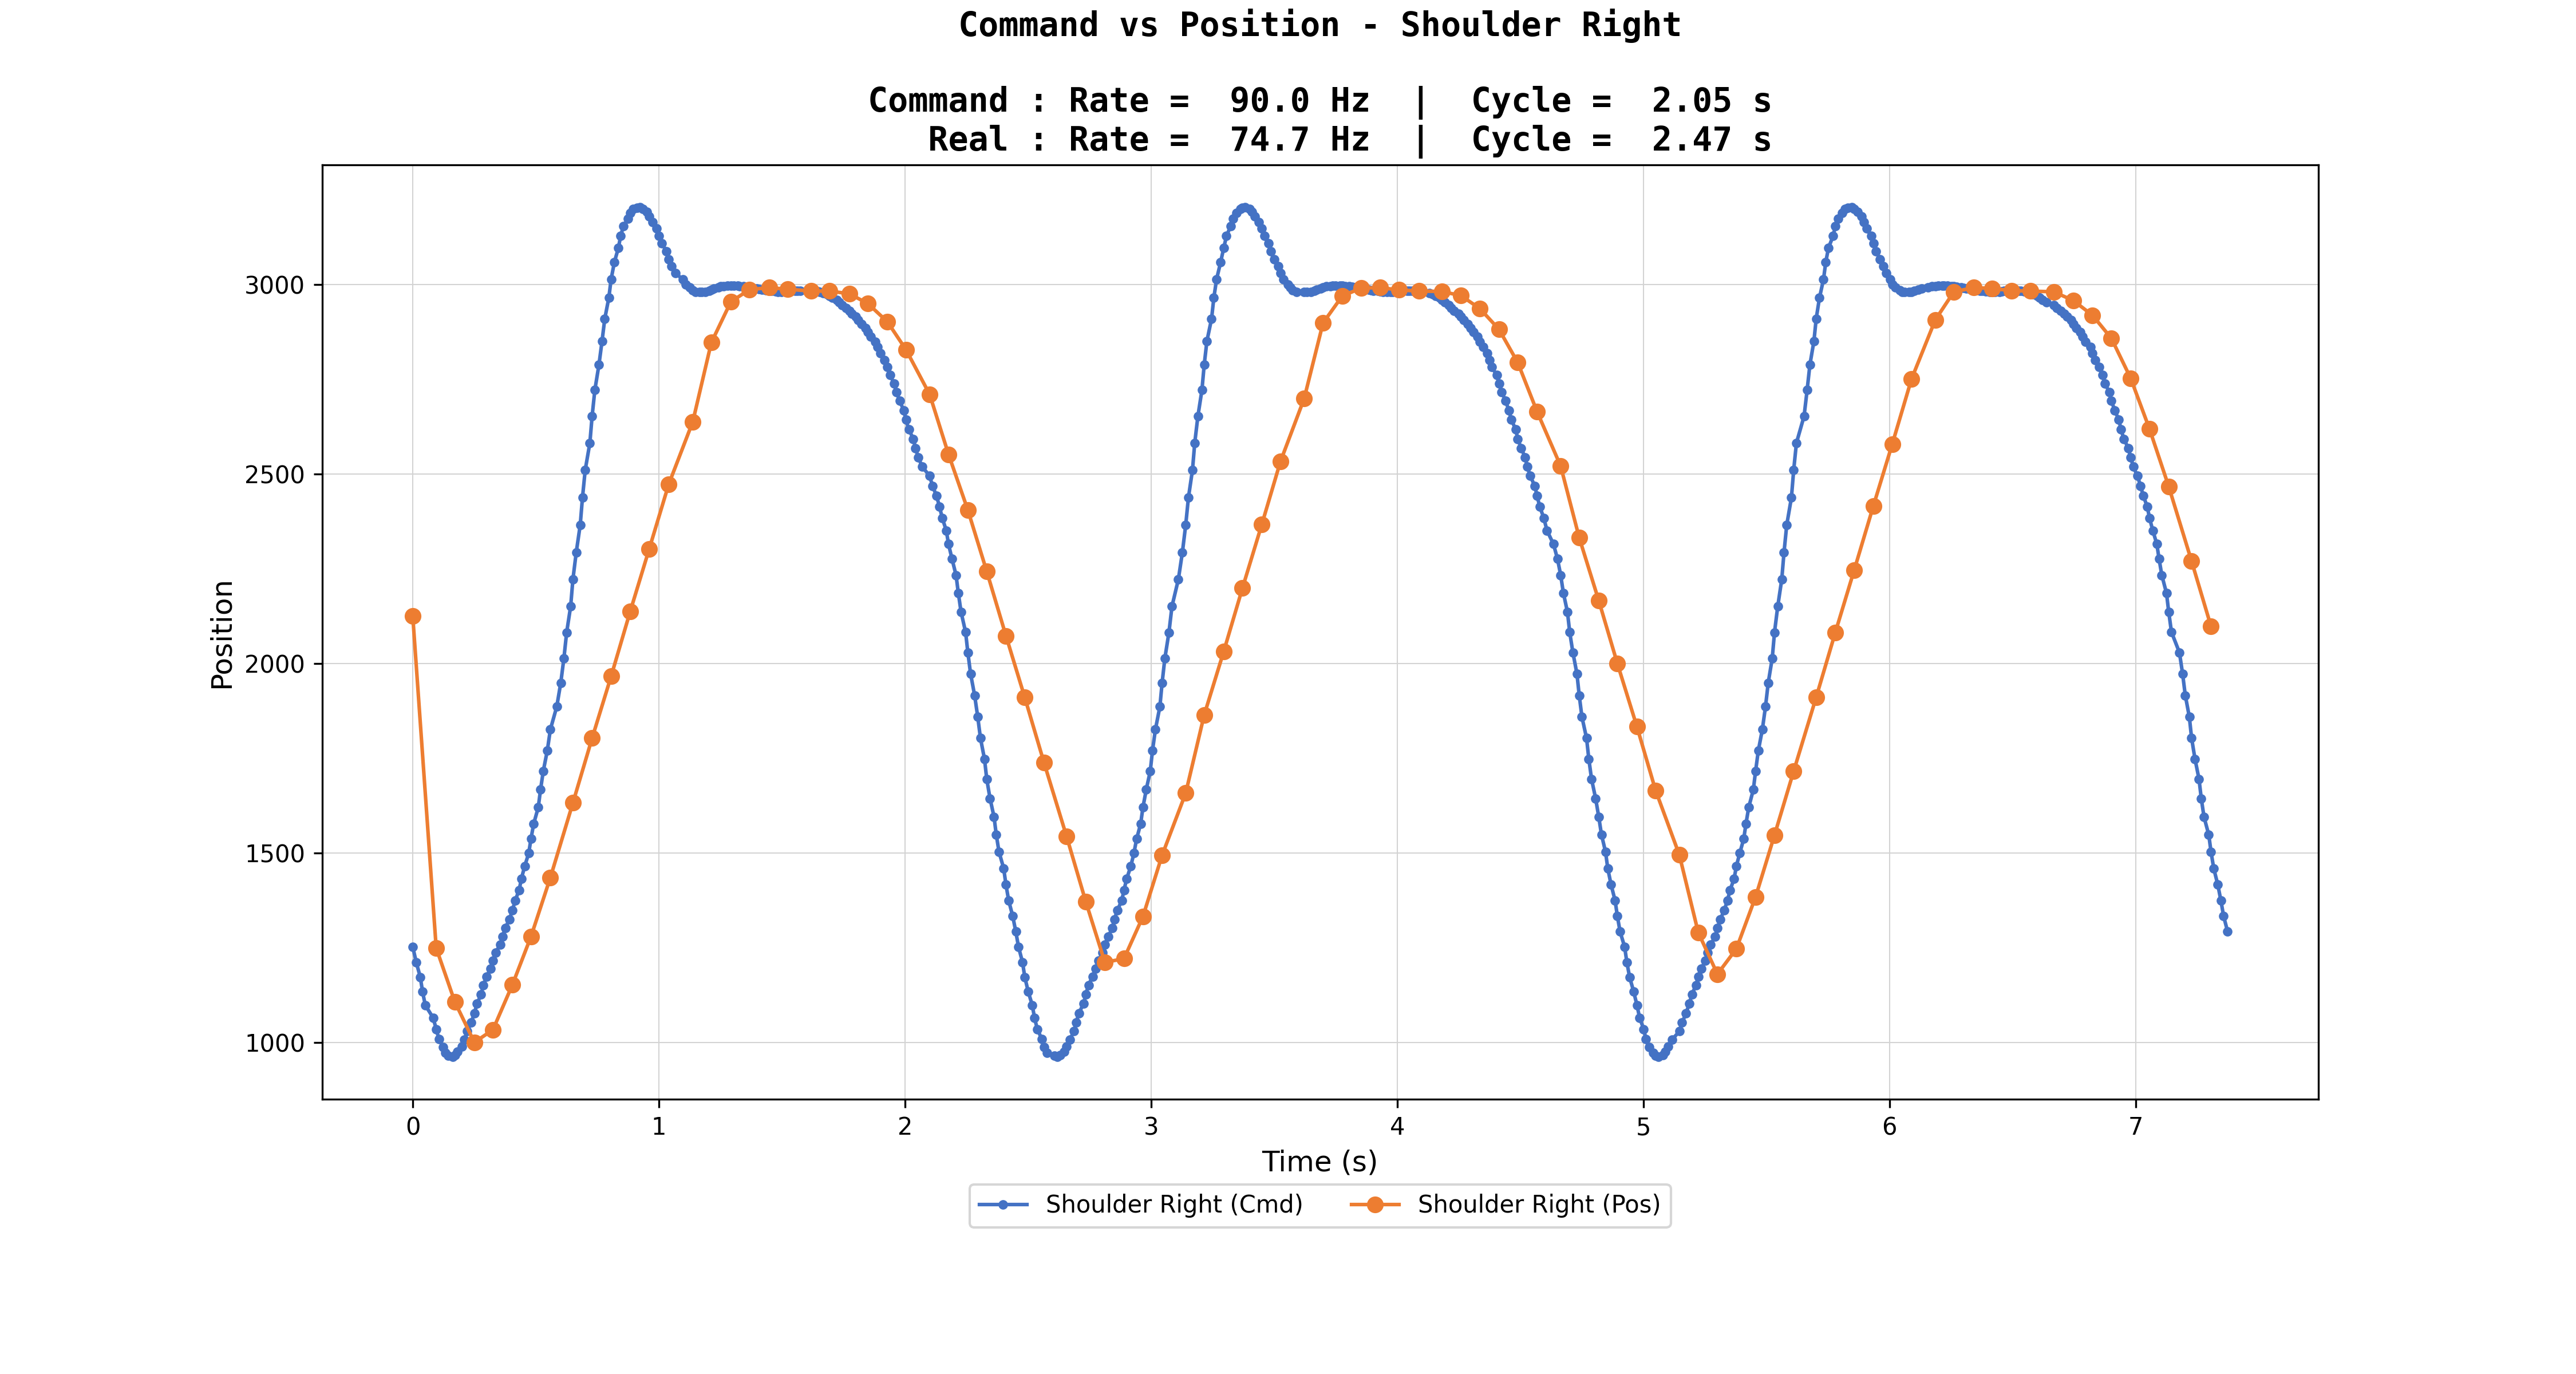
\includegraphics[width=0.8\textwidth]{graphiques/202607141616_ID_4_Spline_Cubic_Pure_90Hz.png}
    \caption{Interpolation naturelle à 90 Hz.}
    \label{fig:spline_nat_90}
\end{figure}

Cependant, la fragilité de cette approche apparaît dès lors que l'on s'éloigne de la fréquence de conception en sous-échantillonnant. En passant à 50~Hz, la spline naturelle commence à montrer ses faiblesses. Le graphique de la figure~\ref{fig:spline_nat_50} met en évidence un décalage bien visible à la fin du cycle : la dernière frame interpolée ne parvient plus à rejoindre proprement la première frame du cycle suivant, créant un saut de consigne.

\begin{figure}[htbp]
    \centering
    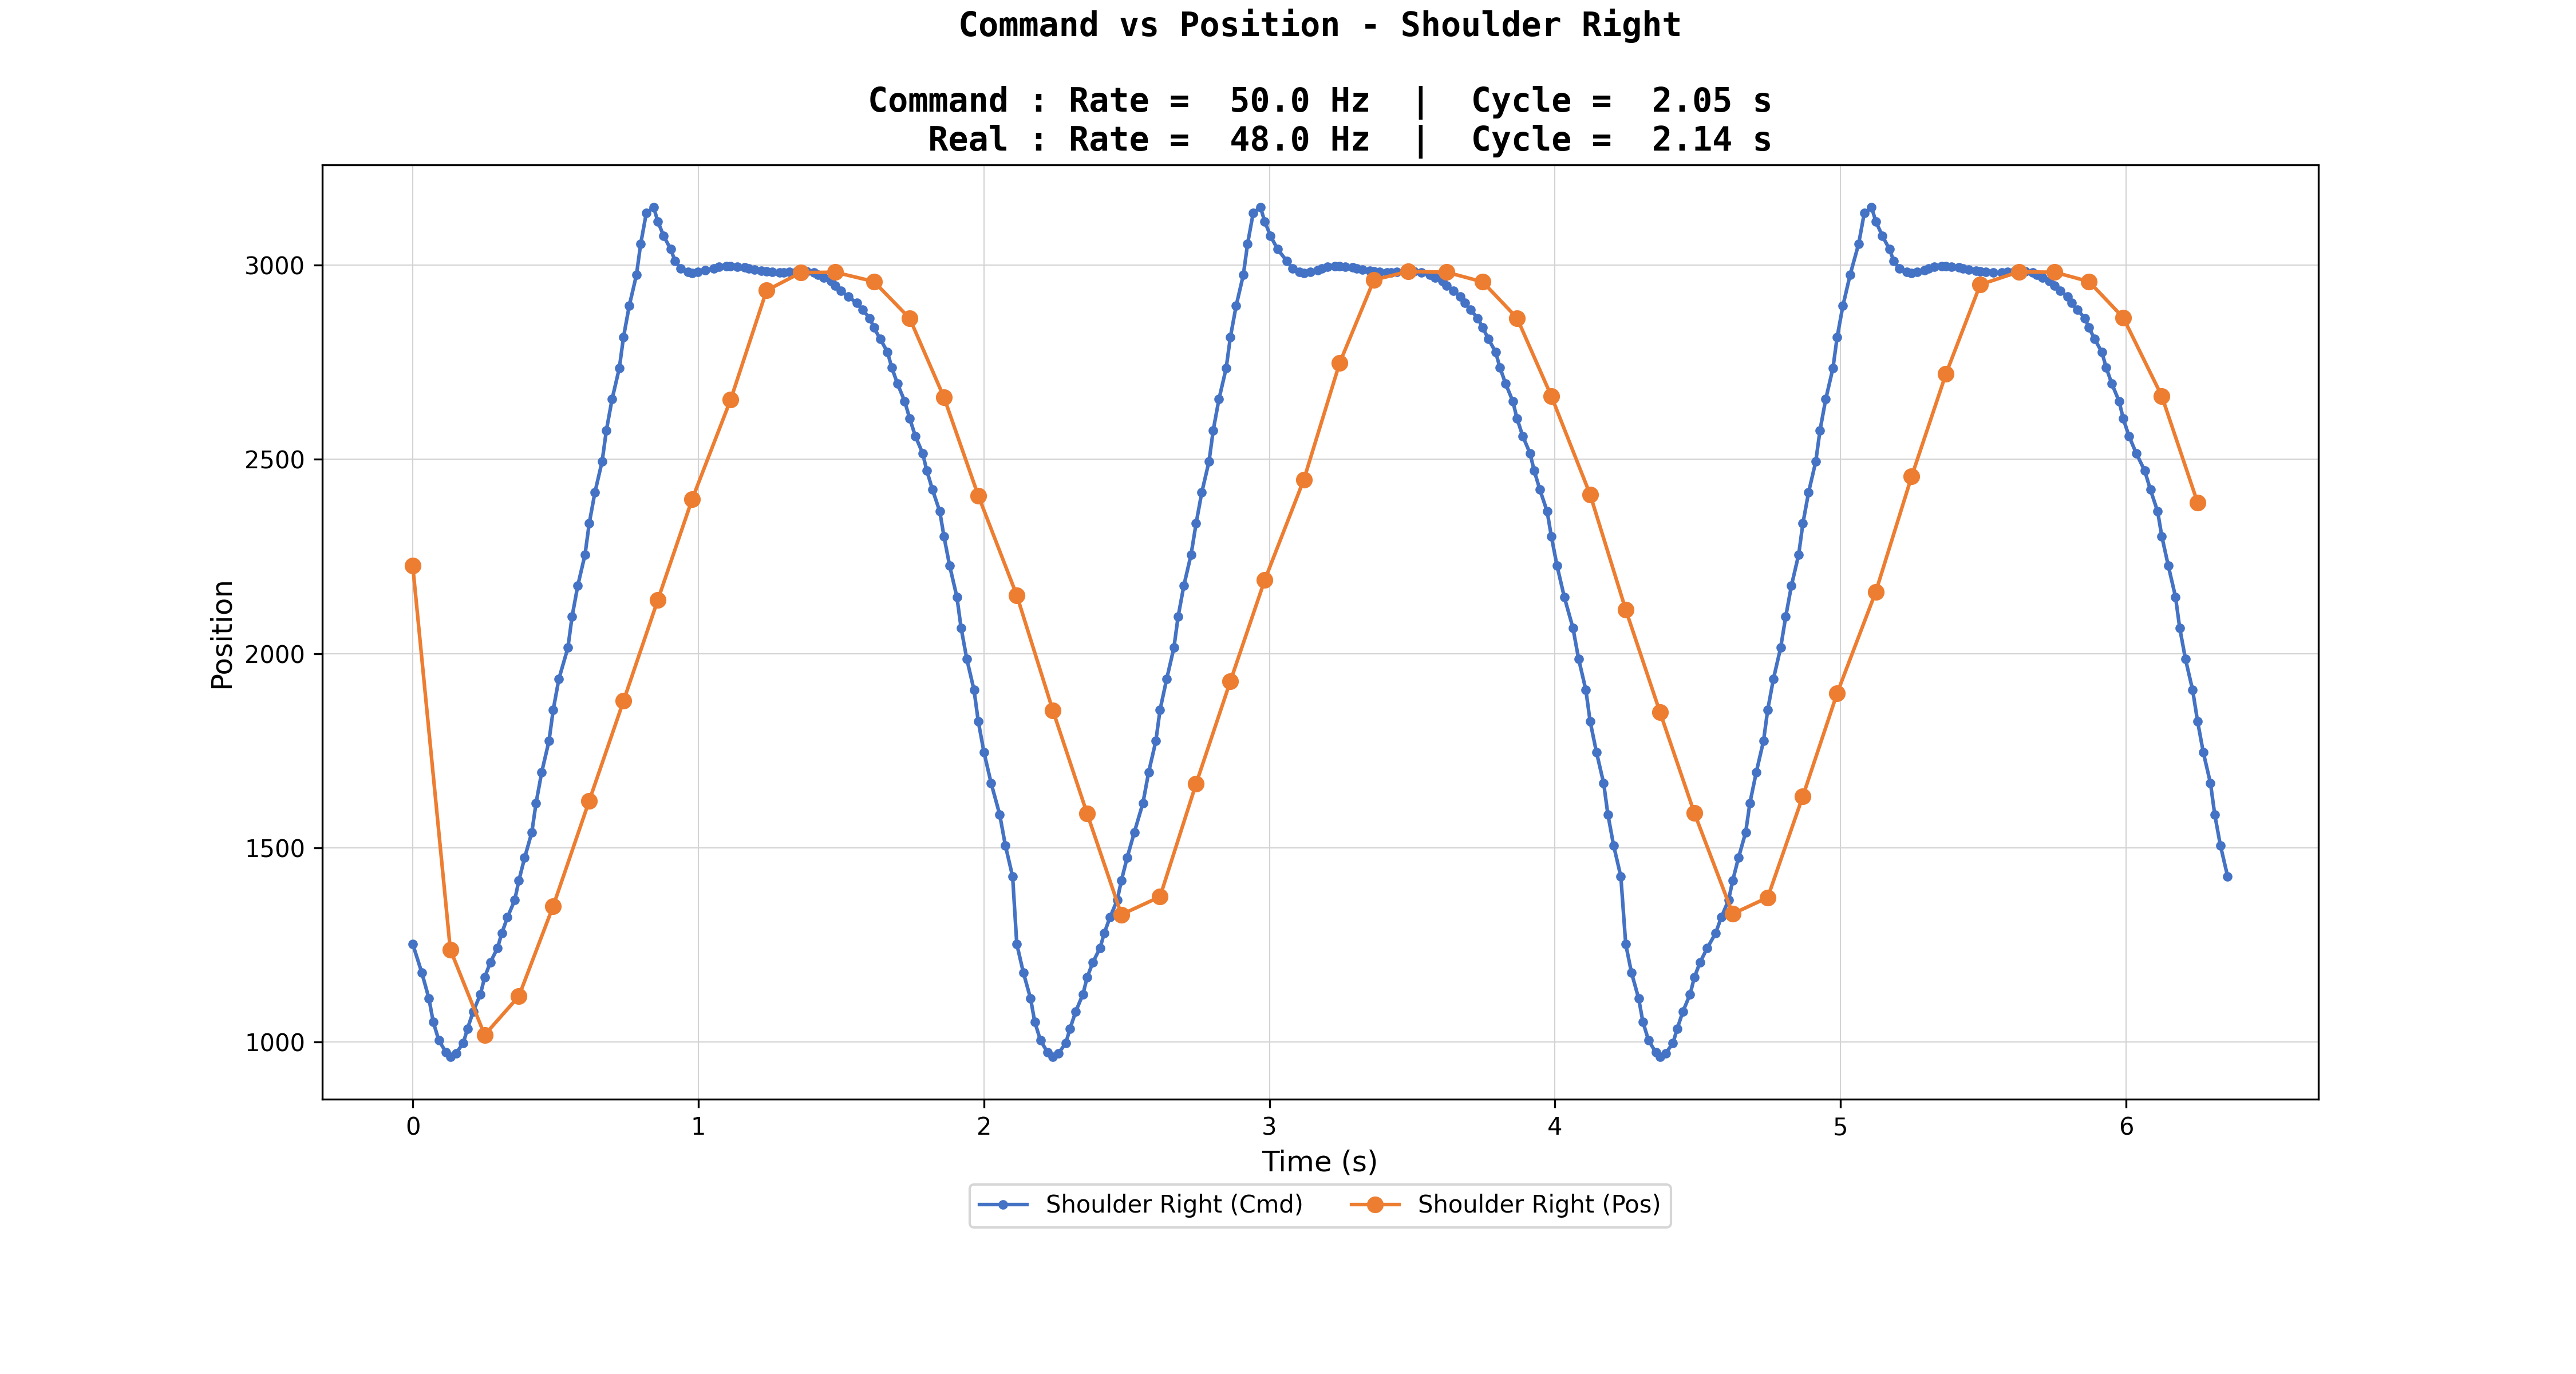
\includegraphics[width=0.8\textwidth]{graphiques/202607141612_ID_4_Spline_Cubic_Pure_50Hz.png}
    \caption{Interpolation naturelle à 50 Hz.}
    \label{fig:spline_nat_50}
\end{figure}

Le problème s'accentue drastiquement aux très basses fréquences. À 36~Hz, soit la moitié de la fréquence nominale, les conditions limites naturelles faussent complètement la dynamique du mouvement aux extrémités. Comme on peut l'observer sur la figure~\ref{fig:spline_nat_36}, il se produit une chute abrupte de la commande à la fin du cycle (à 2,05 s). Ce décalage massif se traduisait, sur le robot physique, par un à-coup mécanique particulièrement violent, compromettant l'intégrité de la nage.

\begin{figure}[htbp]
    \centering
    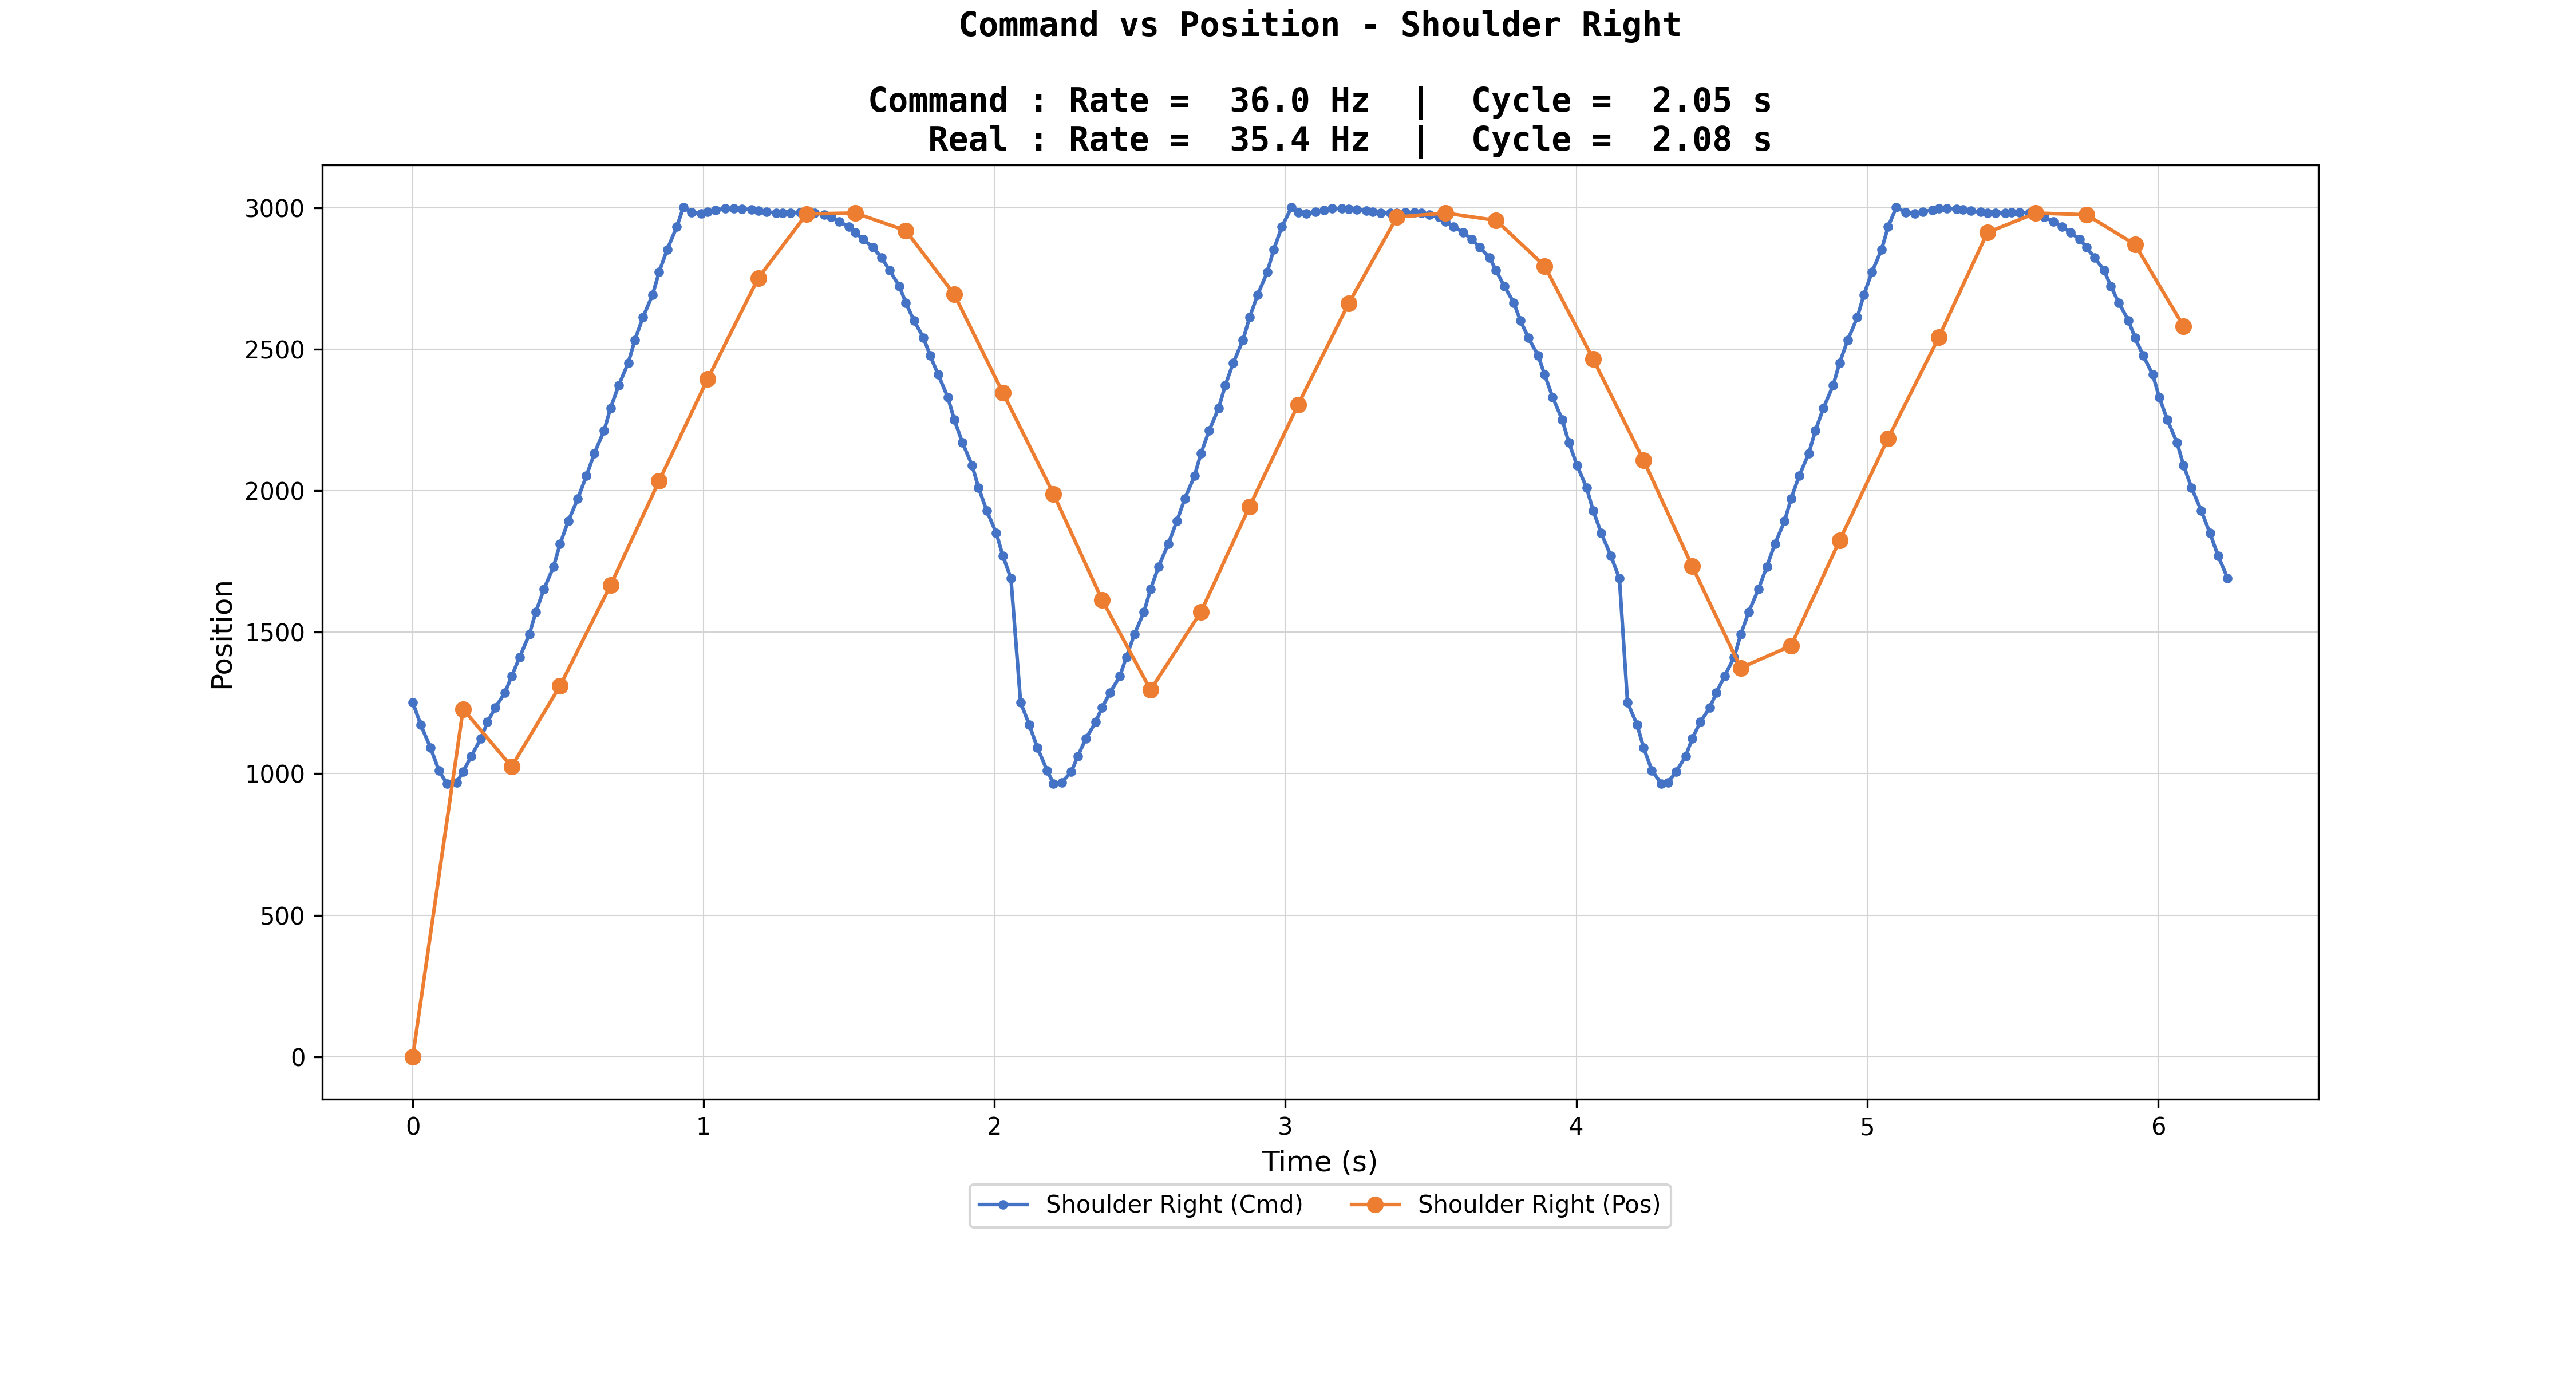
\includegraphics[width=0.8\textwidth]{graphiques/202607141611_ID_4_Spline_Cubic_Pure_36Hz.png}
    \caption{Interpolation naturelle à 36 Hz.}
    \label{fig:spline_nat_36}
\end{figure}

\paragraph{Calcul des dérivées secondes et conditions aux limites périodiques.}
Pour éliminer ce saut de consigne et garantir une boucle fluide, les inconnues $y''_i$ aux nœuds doivent être recalculées différemment. La trajectoire étant destinée à être répétée, elle est modélisée comme une fonction \emph{périodique} de période $N$ : le nœud $x_N$ est identifié au nœud $x_0$ ($y_N \equiv y_0$), et l'on impose à l'interpolant $S$ les conditions aux limites périodiques
\begin{equation}
    S(x_0) = S(x_N), \qquad S'(x_0) = S'(x_N), \qquad S''(x_0) = S''(x_N)
    \label{eq:periodiques}
\end{equation}
qui garantissent la continuité de la position, de la vitesse \emph{et} de l'accélération au passage d'un cycle au suivant. La continuité de la dérivée première fournit, avec un pas uniforme $h = 1$, le système de $N$ équations
\begin{equation}
    y''_{i-1} + 4\,y''_i + y''_{i+1} = 6\left(y_{i+1} - 2y_i + y_{i-1}\right)
    \qquad i = 0,\dots,N-1
    \label{eq:systeme-cyclique}
\end{equation}
où tous les indices sont pris modulo $N$. Sous forme matricielle, la périodicité introduit deux termes de couplage aux coins de la matrice, qui devient \emph{tridiagonale cyclique} :
\begin{equation}
    \begin{pmatrix}
        4 & 1 &        &        & 1 \\
        1 & 4 & 1      &        &   \\
          & \ddots & \ddots & \ddots &   \\
          &        & 1      & 4      & 1 \\
        1 &        &        & 1      & 4
    \end{pmatrix}
    \begin{pmatrix} y''_0 \\ y''_1 \\ \vdots \\ y''_{N-2} \\ y''_{N-1} \end{pmatrix}
    =
    6\begin{pmatrix}
        y_1 - 2y_0 + y_{N-1} \\
        y_2 - 2y_1 + y_0 \\
        \vdots \\
        y_{N-1} - 2y_{N-2} + y_{N-3} \\
        y_0 - 2y_{N-1} + y_{N-2}
    \end{pmatrix}
    \label{eq:matrice-cyclique}
\end{equation}
Ce système n'est plus strictement tridiagonal, mais il se résout toujours en $\mathcal{O}(N)$ grâce à la formule de \textsc{Sherman--Morrison} : la matrice $A$ de~\eqref{eq:matrice-cyclique} s'écrit comme une correction de rang~1 d'une matrice tridiagonale ordinaire $T$,
\begin{equation}
    A = T + u\,v^{\mathsf{T}}, \qquad
    u = (\gamma,\, 0,\, \dots,\, 0,\, 1)^{\mathsf{T}}, \qquad
    v = (1,\, 0,\, \dots,\, 0,\, 1/\gamma)^{\mathsf{T}}
\end{equation}
avec $\gamma = -4$ (choix conventionnel assurant le bon conditionnement de $T$). 

\subsection{Résolution du système cyclique}

\paragraph{Décomposition de Sherman--Morrison et algorithme de Thomas :} Le système~\eqref{eq:matrice-cyclique} n'est pas tridiagonal à cause des deux coefficients de coin $A_{0,N-1} = A_{N-1,0} = 1$. On l'écrit comme une perturbation de rang~1 d'une matrice tridiagonale ordinaire $T$ :
\begin{equation}
    A = T + u\,v^{\mathsf{T}} \qquad
    u = \begin{pmatrix} \gamma \\ 0 \\ \vdots \\ 0 \\ 1 \end{pmatrix} \qquad
    v = \begin{pmatrix} 1 \\ 0 \\ \vdots \\ 0 \\ 1/\gamma \end{pmatrix}
    \qquad \gamma = -4
    \label{eq:sherman-morrison-setup}
\end{equation}
où $\gamma$ est un paramètre libre choisi de sorte que $T$ reste bien conditionnée (ici $\gamma = -4$, l'opposé du terme diagonal courant). Le produit $u\,v^{\mathsf{T}}$ ne modifie que les quatre coins de la matrice :
\begin{equation}
    (u\,v^{\mathsf{T}})_{0,0} = \gamma, \quad
    (u\,v^{\mathsf{T}})_{0,N-1} = \gamma/\gamma = 1, \quad
    (u\,v^{\mathsf{T}})_{N-1,0} = 1, \quad
    (u\,v^{\mathsf{T}})_{N-1,N-1} = 1/\gamma
\end{equation}
si bien que $T = A - u\,v^{\mathsf{T}}$ est \emph{exactement} tridiagonale, de diagonale
\begin{equation}
    T_{i,i} =
    \begin{cases}
        4 - \gamma = 8 & \text{si } i = 0, \\[2pt]
        4 - \dfrac{1}{\gamma} = 4{,}25 & \text{si } i = N-1, \\[6pt]
        4 & \text{sinon,}
    \end{cases}
    \qquad T_{i,i-1} = T_{i,i+1} = 1
    \label{eq:T-diag}
\end{equation}
et de sous/sur-diagonales toutes égales à~1 (indices intérieurs). La formule de Sherman--Morrison donne alors la solution de $A\,y'' = d$ à partir de deux résolutions tridiagonales \emph{ordinaires} :
\begin{equation}
    T z = d, \qquad T w = u, \qquad
    y'' = z - \frac{v^{\mathsf{T}} z}{1 + v^{\mathsf{T}} w}\; w
    \label{eq:sherman-morrison-solution}
\end{equation}
où, compte tenu de la forme creuse de $v$, le produit scalaire se réduit à $v^{\mathsf{T}} z = z_0 + z_{N-1}/\gamma$ (et de même pour $v^{\mathsf{T}} w$) : seules les composantes de tête et de queue des vecteurs interviennent, aucune matrice n'est jamais formée explicitement.\\

Chacun des deux systèmes tridiagonaux $Tz=d$ et $Tw=u$ est résolu par l'\emph{algorithme de Thomas}, variante de l'élimination de Gauss spécialisée aux matrices tridiagonales et de complexité $\mathcal{O}(N)$ (au lieu de $\mathcal{O}(N^3)$ pour une inversion générale). Pour un système générique $T x = r$ de diagonale $T_{i,i}$ et de sous/sur-diagonales unitaires, l'algorithme se déroule en deux passes :

\begin{enumerate}
    \item \textbf{Balayage avant (élimination) :} on élimine la sous-diagonale ligne après ligne, en substituant dans chaque équation le pivot de la ligne précédente. On initialise
    \begin{equation}
        c'_0 = \frac{1}{T_{0,0}}, \qquad x_0 = \frac{r_0}{T_{0,0}}
    \end{equation}
    puis, pour $i = 1, \dots, N-1$, en notant que le pivot effectif de la ligne $i$ après élimination de la colonne $i-1$ vaut $m_i = T_{i,i} - c'_{i-1}$ (la sur-diagonale de la ligne $i-1$ valant~1) :
    \begin{equation}
        m_i = T_{i,i} - c'_{i-1}, \qquad
        c'_i = \frac{1}{m_i}, \qquad
        x_i = \frac{r_i - x_{i-1}}{m_i}
        \label{eq:thomas-forward}
    \end{equation}
    À l'issue de cette passe, le système a été ramené à une forme \emph{bidiagonale supérieure} équivalente.
    \item \textbf{Substitution arrière :} on parcourt les indices en sens inverse pour propager la correction due aux termes sur-diagonaux, restés en suspens lors du balayage avant :
    \begin{equation}
        x_i \leftarrow x_i - c'_i\, x_{i+1}, \qquad i = N-2,\, N-3,\, \dots,\, 0
        \label{eq:thomas-backward}
    \end{equation}
\end{enumerate}
Les deux passes ne coûtent chacune que $\mathcal{O}(N)$ opérations arithmétiques, et la matrice $T$ n'est factorisée qu'une seule fois. Le coût total reste donc linéaire en $N$, ce qui autorise le recalcul instantané de la trajectoire des 21 articulations à chaque modification des paramètres.

\paragraph{Rééchantillonnage périodique et raccord de cycle.} Une fois le vecteur $y''$ connu, la courbe fermée est évaluée en $F$ points uniformément répartis sur une période, \emph{en excluant} le point de raccord (qui appartient au cycle suivant) :
\begin{equation}
    x_k = k\,\frac{N}{F}, \qquad k = 0,\, 1,\, \dots,\, F-1
\end{equation}
de sorte que le nombre de frames produites respecte exactement $F = f_{\mathrm{Hz}} \times T_{\mathrm{cycle}}$ et que la frame suivante ($k = F$, première frame du cycle suivant) tombe précisément sur $S(x_N) = y_0$. 

\paragraph{Analyse des performances de la Spline Périodique.}
Cette nouvelle formulation mathématique vient résoudre le problème de discontinuité à la source. En reprenant le cas critique d'un sous-échantillonnage à 36~Hz, la figure~\ref{fig:spline_per_36} démontre parfaitement la réussite de la méthode. La courbe de commande (en bleu) anticipe la fin du cycle et se raccorde de manière parfaitement lisse au début du cycle suivant. La transition, au bout de 2 secondes, s'effectue sans aucune rupture de pente, éliminant définitivement les à-coups mécaniques.

\begin{figure}[htbp]
    \centering
    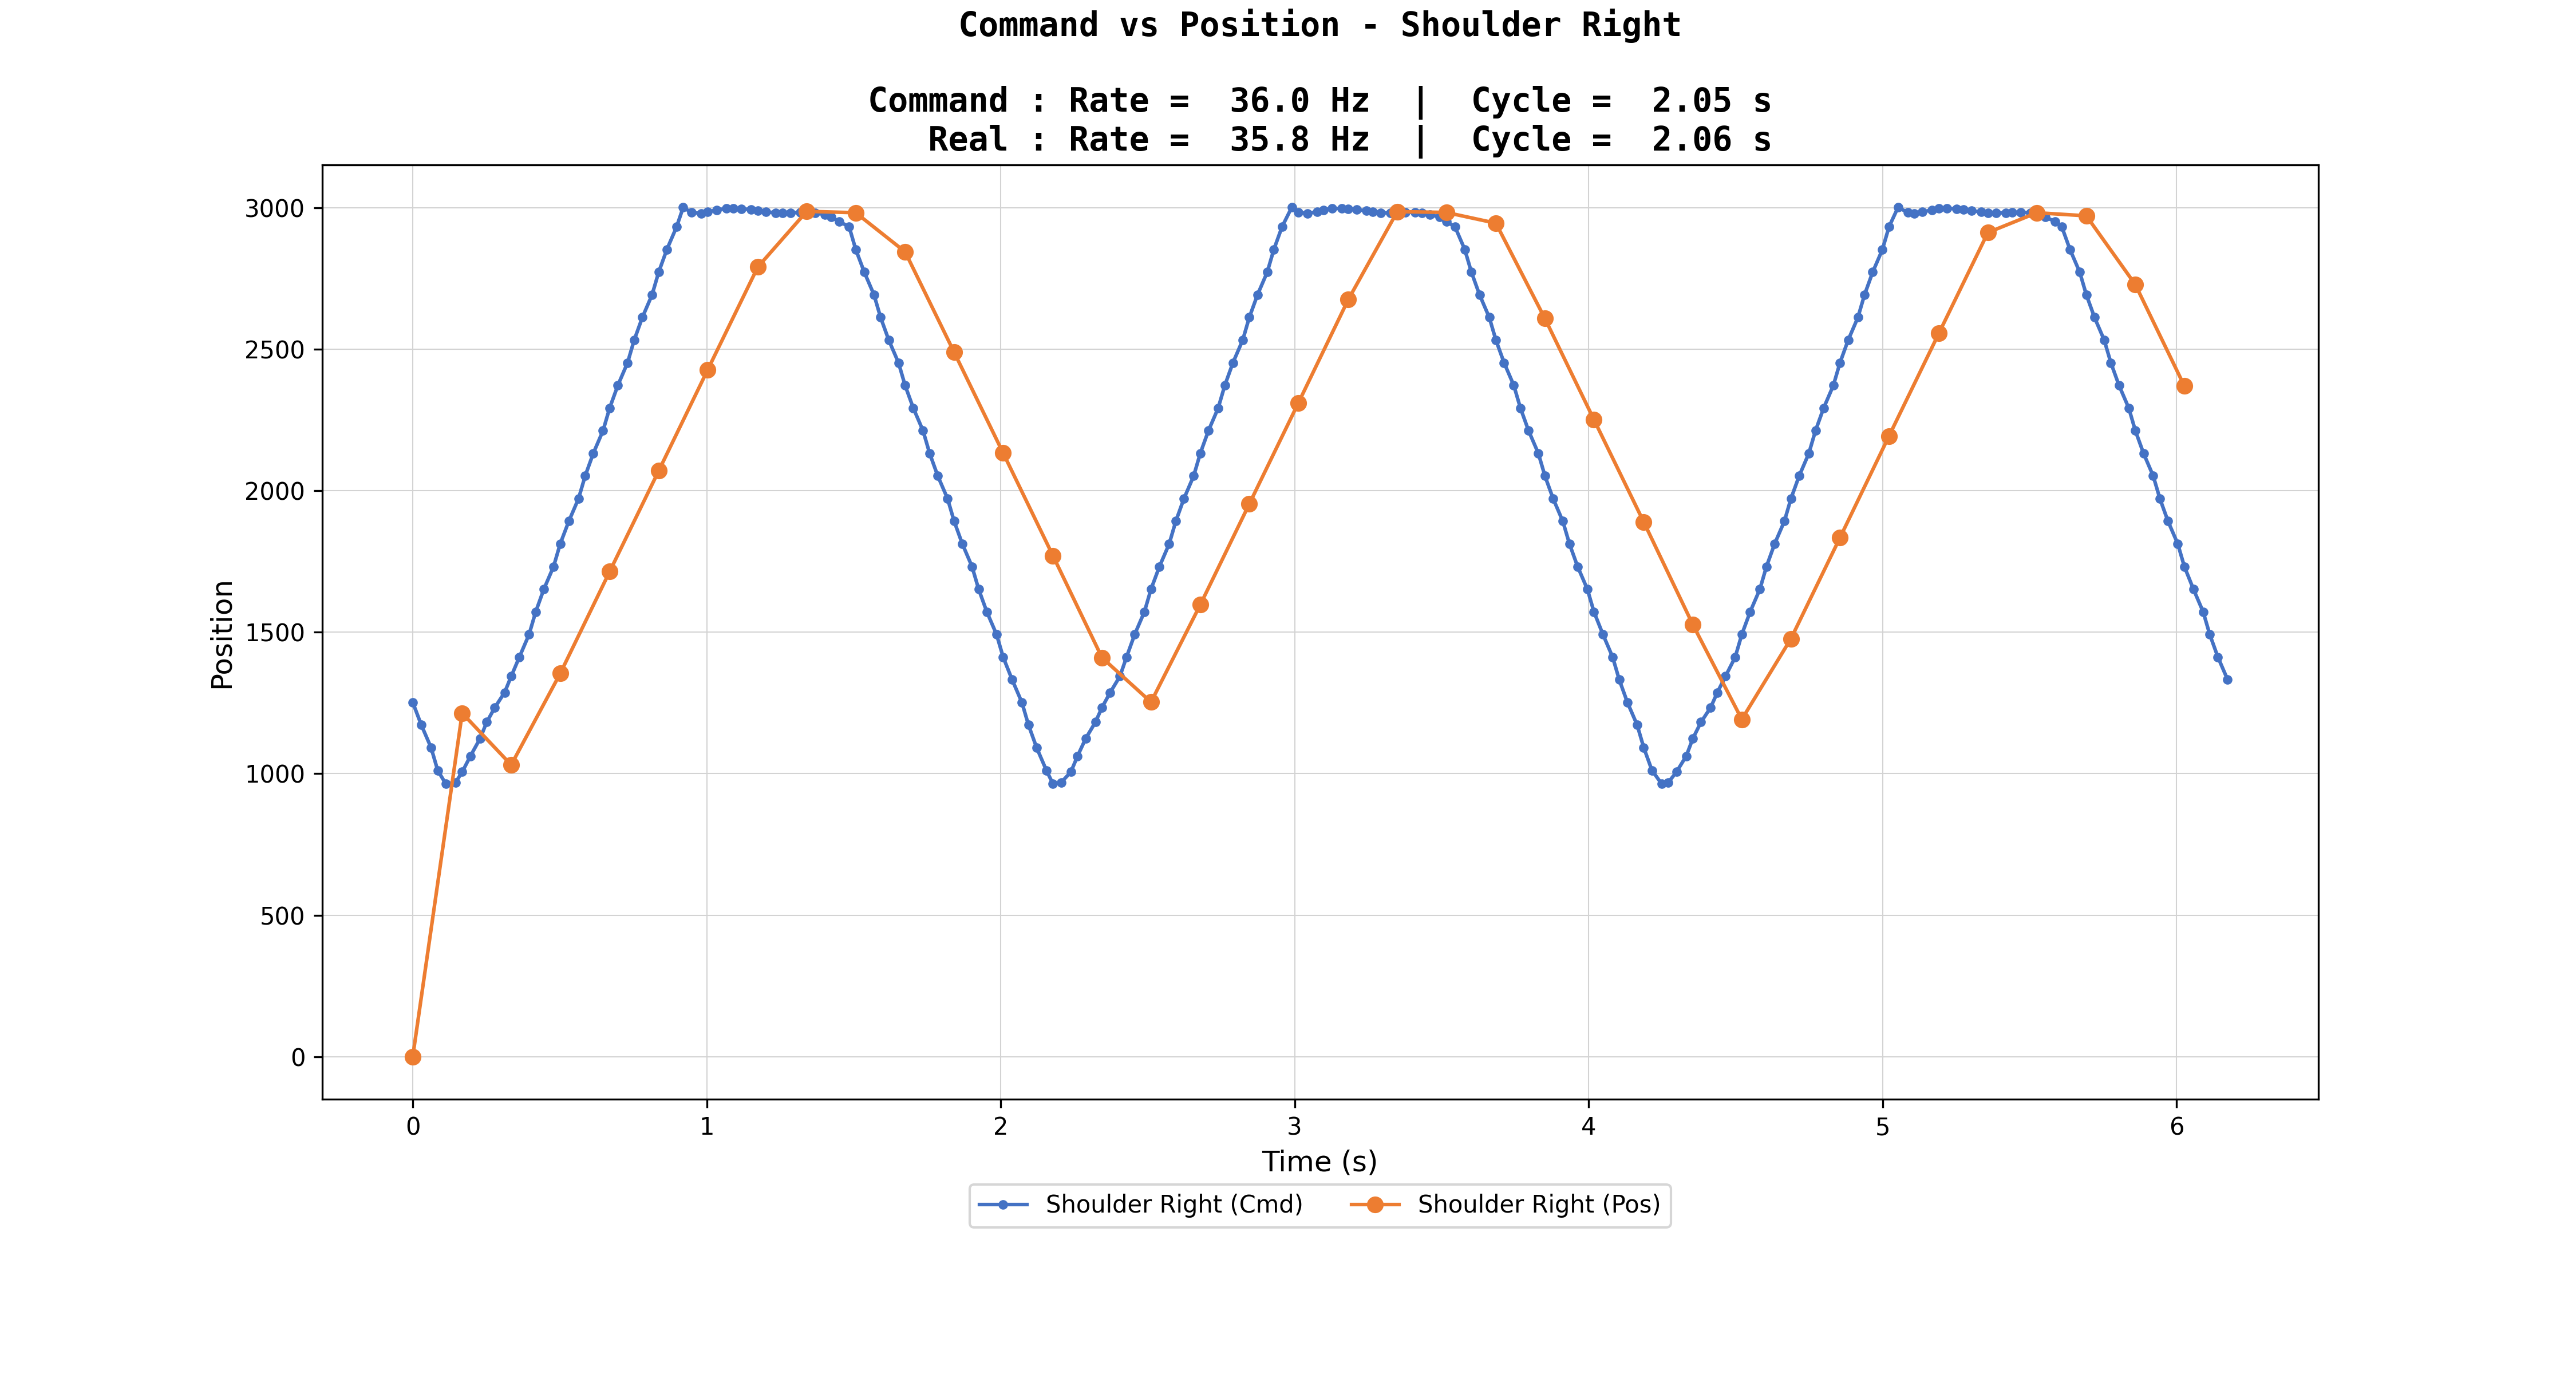
\includegraphics[width=0.8\textwidth]{graphiques/202607141717_ID_4_Spline_Cubique_Periodique_36Hz.png}
    \caption{Interpolation périodique à 36 Hz.}
    \label{fig:spline_per_36}
\end{figure}

Cette continuité structurelle se confirme naturellement à des fréquences intermédiaires. La figure~\ref{fig:spline_per_50} montre qu'à 50~Hz, là où la spline naturelle laissait apparaître un décrochage visible, la spline périodique assure une boucle fermée impeccable. Le signal s'enchaîne de manière homogène sur des cycles infinis.

\begin{figure}[htbp]
    \centering
    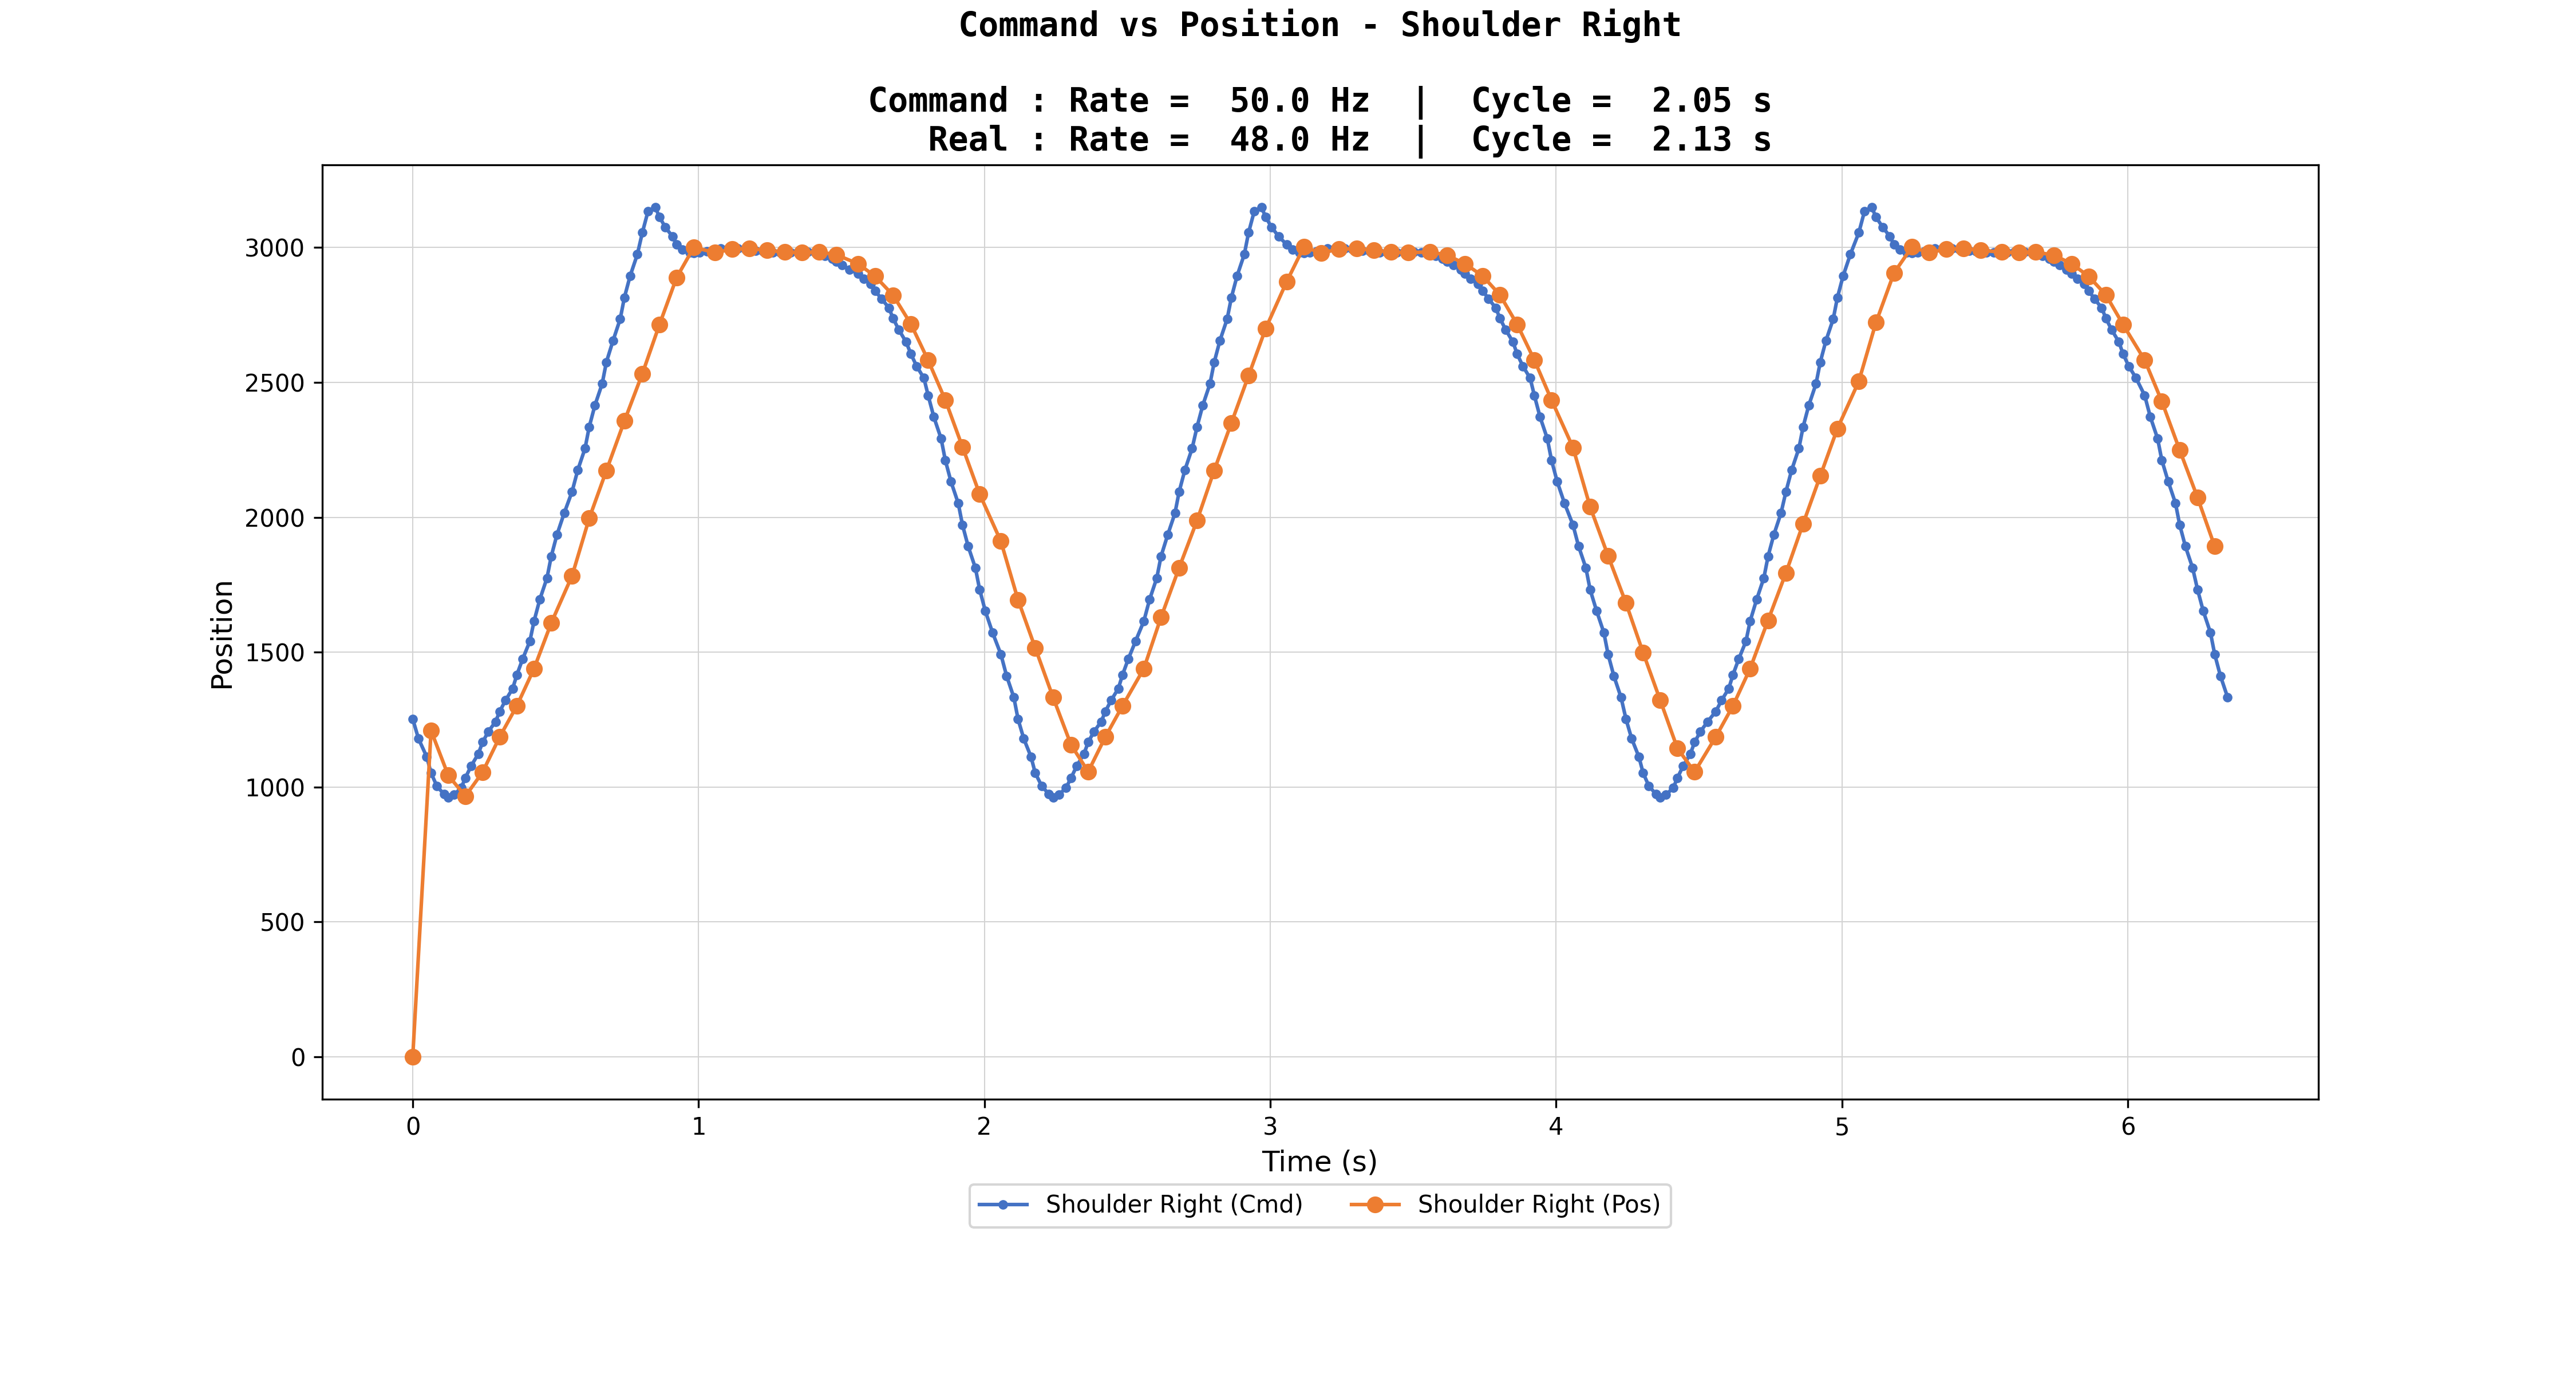
\includegraphics[width=0.8\textwidth]{graphiques/202607141720_ID_4_Spline_Cubique_50Hz.png}
    \caption{Interpolation périodique à 50 Hz.}
    \label{fig:spline_per_50}
\end{figure}

Enfin, à haute fréquence (90~Hz), la méthode maintient la très haute fidélité du mouvement tout en garantissant un raccord parfait aux limites, comme l'illustre la figure~\ref{fig:spline_per_90}. 

\begin{figure}[htbp]
    \centering
    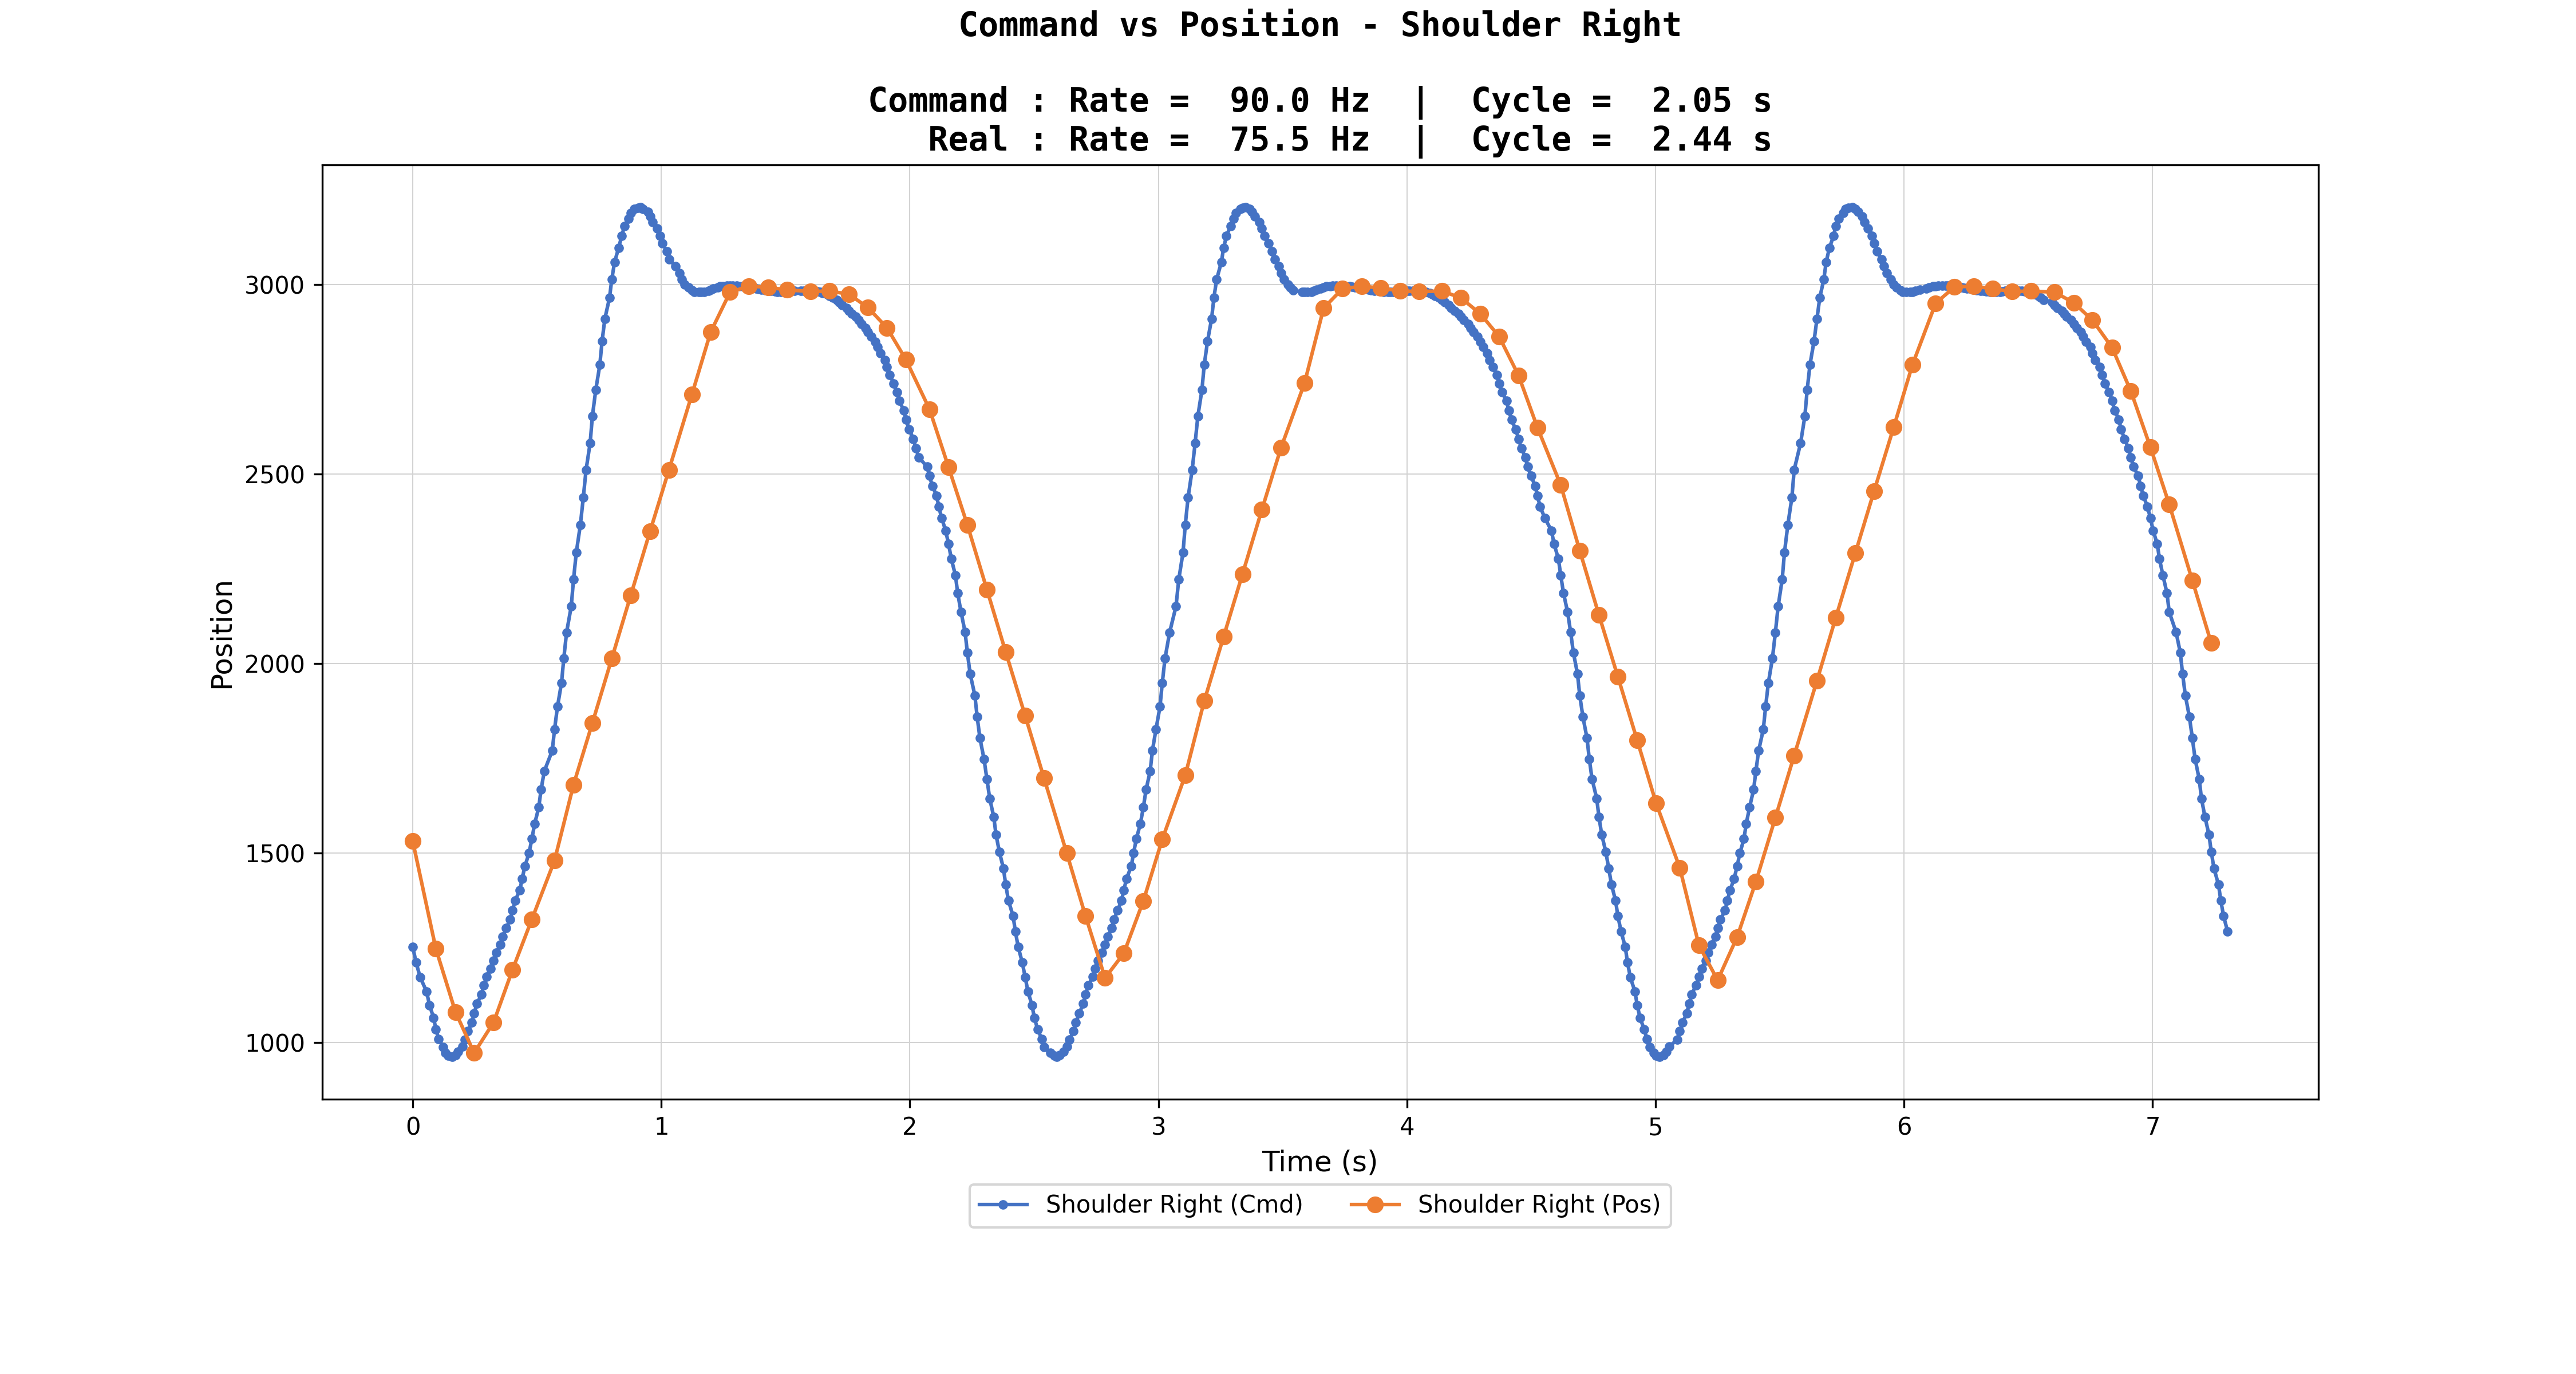
\includegraphics[width=0.8\textwidth]{graphiques/202607141725_ID_4_Spline_Cubique_Periodique_90Hz.png}
    \caption{Interpolation périodique à 90 Hz.}
    \label{fig:spline_per_90}
\end{figure}

Par construction de l'interpolant périodique~\eqref{eq:periodiques}, la position, la vitesse et l'accélération sont rigoureusement continues au rebouclage : le raccord entre deux cycles consécutifs est de classe $\mathcal{C}^2$, au même titre que n'importe quel point intérieur de la trajectoire. L'élan du mouvement de nage est ainsi intégralement conservé d'un cycle au suivant, et les à-coups moteurs au rebouclage sont éliminés non plus approximativement mais exactement. En pratique, la discontinuité résiduelle de vitesse mesurée au raccord est inférieure à la variation de vitesse maximale observée à l'intérieur du cycle. Notons enfin que si le fichier source se termine explicitement par une copie de sa première frame, ce doublon est retiré avant l'ajustement afin de ne pas introduire de nœud double dans la période.\\

\subsection{Rampe Minimum-Jerk} 

Pour le déplacement vers la position initiale, le firmware C++ génère désormais une trajectoire d'approche polynomiale de degré 5 (\textit{minimum-jerk}). L'équation temporelle normalisée est :
\begin{equation}
s(t) = 6t^5 - 15t^4 + 10t^3, \quad t \in [0,1]
\end{equation}
La consigne articulaire à l'instant $k$ est alors calculée de manière fluide par :
\begin{equation}
q_k = q_{start} + s\left(\frac{k}{g_{rampSteps}}\right) \cdot (q_{goal} - q_{start})
\end{equation}
Cette sécurisation logicielle est couplée à un bridage matériel temporaire de la vitesse via les registres Dynamixel comme l'illustre le tableau \ref{tab:hardware_profile}.
    
\begin{table}[h]
\centering
\begin{tabular}{|l|c|l|}
\hline
\textbf{Registre} & \textbf{Adresse} & \textbf{Valeur lors de l'initialisation} \\ \hline
\texttt{Profile Acceleration} & 108 & \texttt{10} (Accélération très douce) \\ \hline
\texttt{Profile Velocity} & 112 & \texttt{40} ($\approx 9$ rpm) \\ \hline
\end{tabular}
\caption{Bridage matériel des actionneurs.}
\label{tab:hardware_profile}
\end{table}

\textbf{Correction de la boucle CPU :} La limitation à 15 Hz a été résolue en séparant drastiquement les appels UART bloquants de la gestion réseau (SSE), et en forçant la réinitialisation des timers matériels de l'ESP32 au lancement du mouvement.

\section{Implémentation d'un contrôleur PID}



\section{Configuration angulaire du SWUMANOID par l'IMU}

Cette section formalise, de manière exhaustive, la chaîne de traitement cinématique retenue pour estimer les angles de \emph{roulis} ($\phi$, autour de l'axe longitudinal $X$) et de \emph{lacet} ($\psi$, autour de la verticale $Z$) du robot SWUMANOID à partir de la centrale inertielle (IMU) logée dans l'AtomS3R. La centrale ne fournit qu'un accéléromètre trois axes $\mathbf{a}=(A_x,A_y,A_z)^{\mathsf T}$ et un gyroscope trois axes $\boldsymbol{\omega}=(G_x,G_y,G_z)^{\mathsf T}$, exprimés dans le repère \emph{carte} $\mathcal{B}$ de l'AtomS3R ; ni quaternion d'attitude ni magnétomètre ne sont transmis.

L'attitude est donc reconstruite intégralement à bord du client, transformée dans le repère du robot $\mathcal{R}$, référencée par une opération de tare, puis lissée. La convention adoptée est \emph{Z-Up} (axe vertical du robot orienté vers le haut), conforme aux standards de la robotique.

\begin{figure}[htbp]
    \centering
    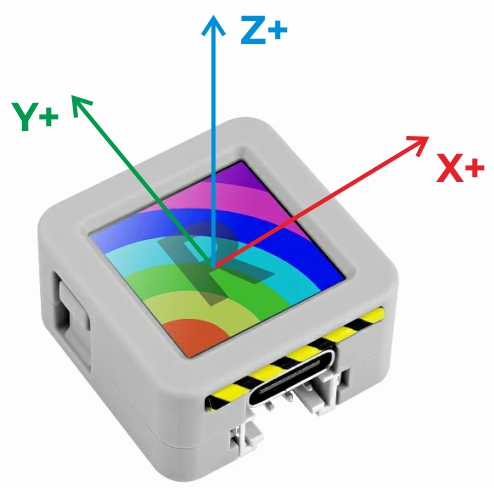
\includegraphics[width=0.45\linewidth]{schemas/IMU-AtomS3R_Defaut_Axes.png}
    \caption{Orientation native des axes de la centrale inertielle (repère $\mathcal{B}$) de l'AtomS3R.}
    \label{fig:imu_axes}
\end{figure}

On note les quaternions unitaires $q=(q_w,q_x,q_y,q_z)$ (partie scalaire d'abord), $\otimes$ le produit de Hamilton, $q^{*}$ le conjugué et, pour un quaternion unitaire, $q^{-1}=q^{*}$. Le repère monde $\mathcal{W}$ est aligné sur la gravité, $\mathbf{z}_{\mathcal{W}}=(0,0,1)^{\mathsf T}$ pointant vers le haut. Les axes par défaut de l'AtomS3R et le repère cible du SWUMANOID sont illustrés respectivement en \textbf{(cf. Figure~\ref{fig:imu_axes})} et \textbf{(cf. Figure~\ref{fig:swumanoid_frame})}.

\newpage

\begin{figure}[htbp]
    \centering
    \begin{subfigure}[b]{\textwidth}
        \centering
        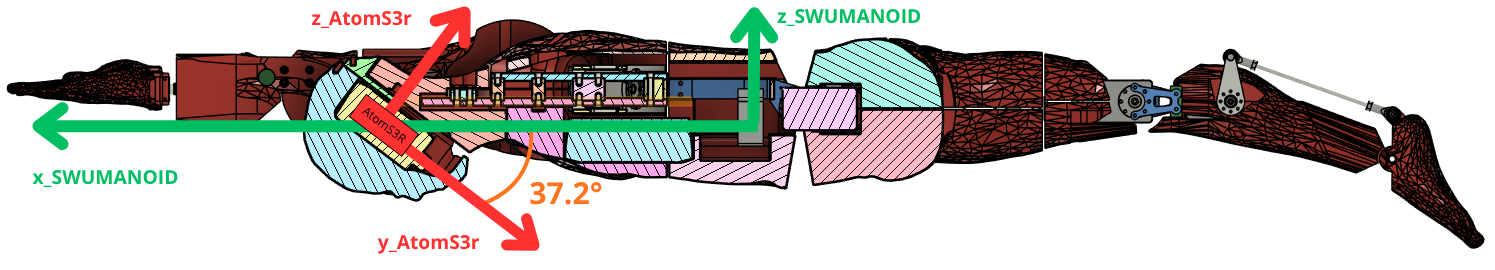
\includegraphics[width=0.95\linewidth]{schemas/AtomS3R_SWUMANOID_orientation_side_view.png}
        \caption{Vue de profil du SWUMANOID.}
    \end{subfigure}
    
    \vspace{0.4cm}
    
    \begin{subfigure}[b]{\textwidth}
        \centering
        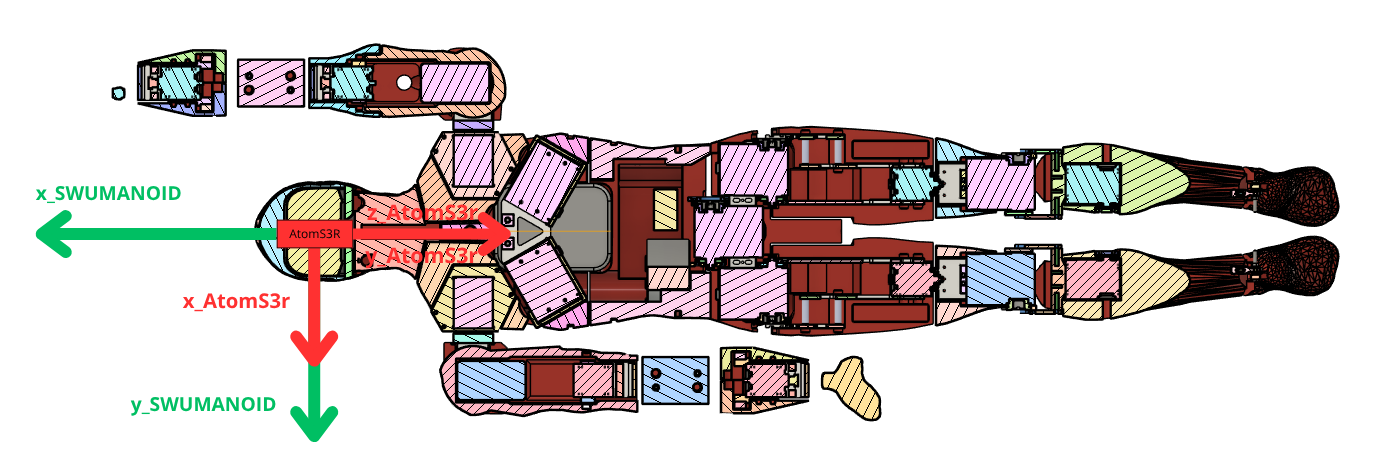
\includegraphics[width=0.95\linewidth]{schemas/AtomS3R_SWUMANOID_orientation_Back_View.png}
        \caption{Vue de dos du SWUMANOID.}
    \end{subfigure}
    \caption{Représentation globale des axes du repère local de l'AtomS3R (en rouge) par rapport au repère cible du robot SWUMANOID $\mathcal{R}$ (en vert).}
    \label{fig:swumanoid_frame}
\end{figure}

\subsection{Acquisition et fusion des données brutes}
\label{subsec:acquisition}

\paragraph{Conditionnement des mesures.}
Le micrologiciel transmet l'accélération en milli-$g$ et la vitesse angulaire en déci-degré par seconde ; les grandeurs physiques sont restituées par
\begin{equation}
\mathbf{a}=\frac{1}{1000}\,\mathbf{a}_{\text{raw}}\ [\,g\,],
\qquad
\boldsymbol{\omega}=\frac{1}{10}\,\boldsymbol{\omega}_{\text{raw}}\ [\,^\circ\!/\mathrm{s}\,]
\end{equation}
Une zone morte est ensuite appliquée composante par composante au gyroscope, afin de neutraliser le bruit de repos responsable de la dérive lente du lacet :
\begin{equation}
\tilde{\omega}_i=
\begin{cases}
0 & \text{si } |\omega_i|<\omega_{\mathrm{db}},\\
\omega_i & \text{sinon,}
\end{cases}
\qquad i\in\{x,y,z\},\quad \omega_{\mathrm{db}}=1{.}2~^\circ\!/\mathrm{s}
\end{equation}

\paragraph{Référence gravitaire (accéléromètre) : socle physique du roulis.}
Au repos, l'accéléromètre mesure la réaction à la pesanteur, soit un vecteur de norme unité (en $g$) colinéaire à la verticale locale. Sa projection sur les axes du repère fournit une estimation \emph{sans dérive} de l'inclinaison. En supposant le capteur quasi statique, la gravité mesurée s'écrit dans $\mathcal B$
\begin{equation}
\mathbf{a}=\mathbf{R}(\phi,\theta)^{\mathsf T}
\begin{pmatrix}0\\0\\1\end{pmatrix}
\end{equation}
ce qui, en développant la matrice de rotation pour un roulis $\phi$ (autour de $X$) et un tangage $\theta$ (autour de $Y$), conduit aux composantes
\begin{equation}
A_x=-\sin\theta,\qquad
A_y=\cos\theta\,\sin\phi,\qquad
A_z=\cos\theta\,\cos\phi
\end{equation}
On en déduit, par élimination et usage de la fonction $\operatorname{arctan2}$ (qui lève l'ambiguïté de quadrant sur $[-\pi,\pi]$), les angles d'inclinaison \emph{instantanés} :
\begin{empheq}[box=\fbox]{align}
\phi_{\text{acc}} &= \operatorname{arctan2}\!\big(A_y,\;A_z\big) \label{eq:roll_acc}\\
\theta_{\text{acc}} &= \operatorname{arctan2}\!\Big(-A_x,\;\sqrt{A_y^{2}+A_z^{2}}\Big) \label{eq:pitch_acc}
\end{empheq}
L'équation~\eqref{eq:roll_acc} constitue le socle physique de l'estimation du roulis. Toutefois, l'accéléromètre présente deux limites structurelles : il est \emph{aveugle au lacet} (la gravité est invariante par rotation autour de la verticale, si bien que $\psi$ n'apparaît dans aucune des équations ci-dessus), et il est fortement bruité dès que le capteur subit une accélération propre (vibrations des 21 moteurs Dynamixel, chocs), le vecteur mesuré n'étant alors plus purement gravitaire.

\paragraph{Complément gyroscopique et cinématique du quaternion.}
Le gyroscope fournit la vitesse angulaire instantanée et permet, par intégration, un suivi fin et à faible latence de l'orientation ; il souffre en revanche d'une dérive cumulative (biais intégré). La démarche de fusion consiste donc à combiner la stabilité long terme de l'accéléromètre~\eqref{eq:roll_acc}--\eqref{eq:pitch_acc} avec la réactivité court terme du gyroscope. Plutôt que de manipuler des angles d'Euler (sujets au blocage de cardan), l'orientation est portée par un quaternion d'attitude $q_{\text{raw}}$ ($\mathcal B\rightarrow\mathcal W$) dont la cinématique obéit à
\begin{equation}
\dot{q}=\tfrac{1}{2}\,q\otimes
\begin{pmatrix}0\\ \boldsymbol{\omega}\end{pmatrix}
\label{eq:kinematics}
\end{equation}
$\boldsymbol{\omega}$ étant exprimé dans le repère corps. L'implémentation intègre~\eqref{eq:kinematics} par la carte exponentielle exacte sur chaque intervalle $\Delta t$ mesuré localement : en posant $\boldsymbol{\omega}$ en $\mathrm{rad/s}$, $\Omega=\lVert\boldsymbol{\omega}\rVert$ et $\mathbf{n}=\boldsymbol{\omega}/\Omega$,
\begin{equation}
\delta q=\Big(\cos\tfrac{\Omega\,\Delta t}{2},\;\mathbf{n}\,\sin\tfrac{\Omega\,\Delta t}{2}\Big),
\qquad
q_{\text{raw}}\leftarrow q_{\text{raw}}\otimes\delta q 
\label{eq:gyro_step}
\end{equation}
La post-multiplication (à droite) traduit le caractère \emph{local} (repère mobile) de la rotation mesurée par le gyroscope.

\paragraph{Initialisation de l'attitude.}
Soit $\hat{\mathbf{u}}=\mathbf{a}/\lVert\mathbf{a}\rVert$ la direction de la pesanteur mesurée dans $\mathcal B$. Le quaternion initial est le plus court arc amenant $\hat{\mathbf{u}}$ sur $\mathbf{z}_{\mathcal W}$ :
\begin{equation}
q_{\text{raw}}^{(0)}=\frac{\big(1+\hat{\mathbf{u}}\cdot\mathbf{z}_{\mathcal W},\;\hat{\mathbf{u}}\times\mathbf{z}_{\mathcal W}\big)}{\big\lVert\big(1+\hat{\mathbf{u}}\cdot\mathbf{z}_{\mathcal W},\;\hat{\mathbf{u}}\times\mathbf{z}_{\mathcal W}\big)\big\rVert}
\label{eq:seed}
\end{equation}
de sorte que l'estimation démarre à plat, le lacet étant fixé arbitrairement à zéro (cap purement relatif).

\paragraph{Filtre complémentaire quaternionique.}
À chaque échantillon, la prédiction gyroscopique~\eqref{eq:gyro_step} est recalée sur la gravité \emph{uniquement lorsque} la mesure est jugée quasi statique, c'est-à-dire $\big|\,\lVert\mathbf{a}\rVert-1\,\big|\le\tau$ avec $\tau=0{.}25\,g$ (ce test écarte les phases d'accélération propre, où la gravité est masquée). La verticale prédite dans le repère corps s'écrit
\begin{equation}
\hat{\mathbf{g}}_{\text{pred}}=q_{\text{raw}}^{-1}\otimes\mathbf{z}_{\mathcal W}\otimes q_{\text{raw}},
\end{equation}
et l'on construit le quaternion de correction $\delta q_c$ réalisant le plus court arc de la verticale \emph{mesurée} $\hat{\mathbf{u}}$ vers la verticale \emph{prédite} $\hat{\mathbf{g}}_{\text{pred}}$ (même forme qu'en~\eqref{eq:seed}). Cette correction n'est appliquée que \emph{partiellement}, par interpolation sphérique depuis l'identité avec un gain $\mu$, puis composée à droite et renormalisée :
\begin{equation}
q_{\text{raw}}\leftarrow\frac{q_{\text{raw}}\otimes\operatorname{Slerp}\!\big(\mathbf{1},\,\delta q_c,\,\mu\big)}{\big\lVert\,\cdot\,\big\rVert},
\qquad \mu=0{.}02 .
\label{eq:complementary}
\end{equation}
Le couple \eqref{eq:gyro_step}--\eqref{eq:complementary} réalise ainsi un \emph{filtre complémentaire} : le gyroscope assure les hautes fréquences, tandis que l'accéléromètre corrige, à gain faible $\mu$, la dérive basse fréquence du roulis et du tangage. Cette structure est fonctionnellement analogue à un filtre de Madgwick (correction par descente de gradient d'une erreur d'alignement gravitaire), ici formulée sous une forme géométrique explicite. Le lacet, dépourvu de référence absolue, n'est jamais corrigé et reste issu de la seule intégration~\eqref{eq:gyro_step} : il est \emph{réversible}, ce qui garantit qu'un retour à la pose physique initiale ramène l'estimation au même état. Le quaternion résultant $q_{\text{raw}}$ représente l'attitude absolue de la carte, $\mathcal B\rightarrow\mathcal W$.

\subsection{Changement de repère}
\label{subsec:calib}

L'AtomS3R n'est pas monté selon les axes anatomiques du SWUMANOID : il est logé dans la tête avec une inclinaison mécanique de $37{.}2^\circ$ \textbf{(cf. Figure~\ref{fig:robot_tilt})}. 

\begin{figure}[htbp]
    \centering
    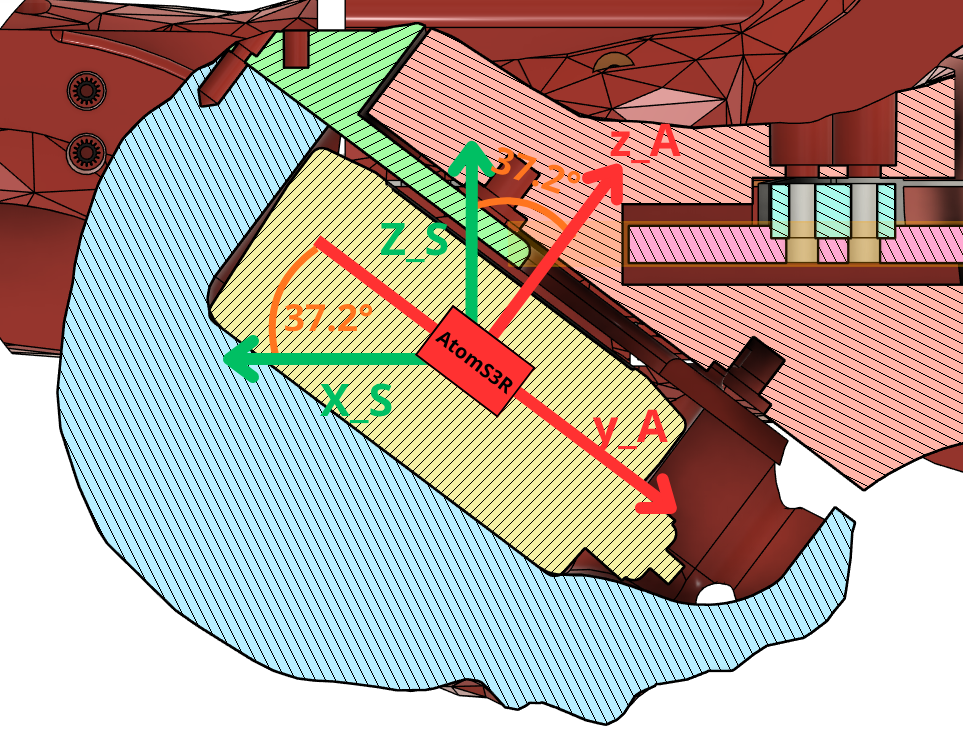
\includegraphics[width=0.6\linewidth]{schemas/AtomS3R_SWUMANOID_orientation_side_view_zoomed.png}
    \caption{Vue détaillée illustrant l'inclinaison mécanique de $37.2^{\circ}$ de l'AtomS3R dans la tête du robot.}
    \label{fig:robot_tilt}
\end{figure}

Pour exprimer l'attitude dans le repère Z-Up du robot $\mathcal R$, on applique une transformation rigide constante $q_{\text{calib}}$ correspondant à la séquence de rotations \emph{intrinsèques} (autour des axes locaux successifs) suivante \textbf{(cf. Figure~\ref{fig:rotation_repere_schema})} :
\begin{enumerate}
  \item $R_1$ : rotation de $+37{.}2^\circ$ autour de l'axe $X$ \emph{initial} de la carte, qui compense l'inclinaison mécanique et redresse l'axe vertical vers le \emph{haut} ;
  \item $R_2$ : rotation de $-90^\circ$ autour du \emph{nouvel} axe $Z'$, qui aligne les axes de la carte sur l'avant ($X$) et la gauche ($Y$) du robot.
\end{enumerate}

\begin{figure}[htbp]
    \centering
    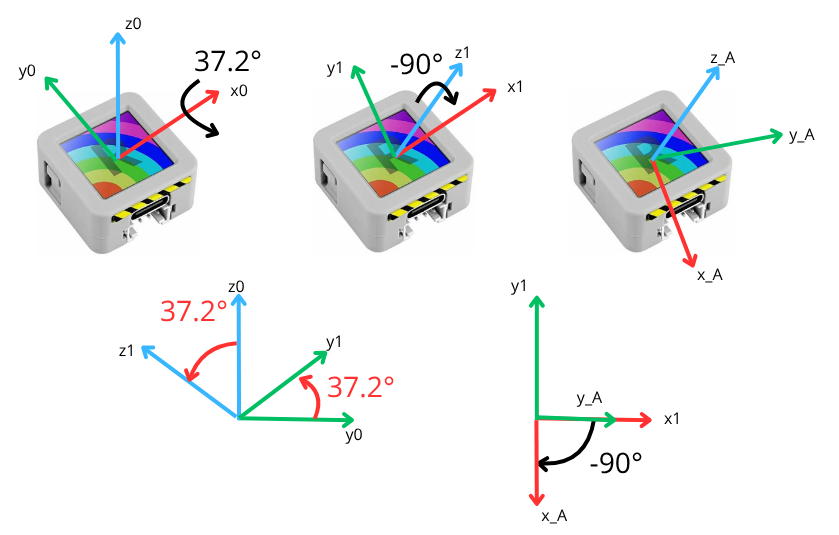
\includegraphics[width=0.8\linewidth]{schemas/AtomS3r_Changement_Repere_Transformation.png}
    \caption{Schéma des rotations intrinsèques successives appliquées pour aligner le repère de la carte sur celui du robot.}
    \label{fig:rotation_repere_schema}
\end{figure}

Le signe négatif de $R_2$ est une conséquence directe de la convention Z-Up : une fois l'axe vertical redressé, la « main » du repère intermédiaire impose une rotation de $-90^\circ$ (et non $+90^\circ$) pour faire coïncider correctement $X$ et $Y$.

\paragraph{Formulation matricielle.}
Avec les matrices de rotation élémentaires
\begin{equation}
R_x(\alpha)=\begin{pmatrix}1&0&0\\0&\cos\alpha&-\sin\alpha\\0&\sin\alpha&\cos\alpha\end{pmatrix},
\qquad
R_z(\beta)=\begin{pmatrix}\cos\beta&-\sin\beta&0\\\sin\beta&\cos\beta&0\\0&0&1\end{pmatrix}
\end{equation}
la composition \emph{intrinsèque} « $R_1$ puis $R_2$ autour de l'axe déjà tourné » s'obtient par \emph{post}-multiplication (et non $R_{z'}R_x$, qui correspondrait à des rotations extrinsèques) :
\begin{equation}
\mathbf{R}_{\text{calib}}=R_x(37{.}2^\circ)\,R_z(-90^\circ),
\qquad
R_z(-90^\circ)=\begin{pmatrix}0&1&0\\-1&0&0\\0&0&1\end{pmatrix}
\label{eq:Rcalib}
\end{equation}

\paragraph{Formulation quaternionique (implémentée).}
Le code n'utilise pas $\mathbf{R}_{\text{calib}}$ mais son quaternion équivalent, afin d'éliminer toute singularité. Avec la paramétrisation axe--angle $q_{\mathbf{n}}(\gamma)=\big(\cos\tfrac{\gamma}{2},\,\mathbf{n}\sin\tfrac{\gamma}{2}\big)$,
\begin{equation}
q_x=q_{\mathbf{e}_x}(37{.}2^\circ)=\big(\cos 18{.}6^\circ,\,\sin 18{.}6^\circ,\,0,\,0\big),
\qquad
q_z=q_{\mathbf{e}_z}(-90^\circ)=\Big(\tfrac{\sqrt{2}}{2},\,0,\,0,\,-\tfrac{\sqrt{2}}{2}\Big)
\end{equation}
\begin{equation}
\boxed{\,q_{\text{calib}}=q_x\otimes q_z\,}
\label{eq:qcalib}
\end{equation}
L'attitude absolue du robot, la monture étant fixée au corps, résulte de la post-multiplication
\begin{equation}
\boxed{\,q_{\text{robot}}=q_{\text{raw}}\otimes q_{\text{calib}}\,}
\label{eq:qrobot}
\end{equation}
On vérifie que l'axe vertical du robot pointe bien vers le haut : la composante verticale de son axe $Z$ dans $\mathcal W$ vaut $\cos(37{.}2^\circ)>0$ (Z-Up), alors que la version antérieure à $+217{.}2^\circ$ donnait $\cos(217{.}2^\circ)<0$ (Z-Down).

\subsection{Opération de tare}
\label{subsec:tare}

L'utilisateur définit la pose courante comme origine $(0,0,0)$. On mémorise l'inverse (conjugué) de l'attitude transformée à l'instant du déclenchement, $q_{\text{robot}}^{(0)}$ :
\begin{equation}
q_{\text{tare}}=\big(q_{\text{robot}}^{(0)}\big)^{-1}=\big(q_{\text{robot}}^{(0)}\big)^{*}
\end{equation}
puis l'attitude affichée est référencée à chaque échantillon par
\begin{equation}
\boxed{\,q_{\text{display}}=q_{\text{tare}}^{-1}\otimes q_{\text{robot}}\,}
\label{eq:qdisplay}
\end{equation}
Par construction, $q_{\text{display}}=\mathbf{1}$ (identité, soit $0^\circ$) lorsque $q_{\text{robot}}=q_{\text{robot}}^{(0)}$ : tout retour à la pose de référence ramène rigoureusement l'affichage à zéro. Ce mécanisme est de surcroît initialisé automatiquement au premier échantillon valide, ce qui garantit un affichage nul au démarrage, indépendamment de l'orientation matérielle de la carte.

\subsection{Extraction des angles d'Euler et filtrage passe-bas}
\label{subsec:extract_filter}

\paragraph{Conversion en angles d'Euler.}
Les angles finaux sont extraits de $q_{\text{display}}$ par conversion en angles de Tait--Bryan selon l'ordre $Z\!-\!Y\!-\!X$. Ce choix est justifié par la structure du problème : dans une décomposition à trois axes, seul l'axe \emph{intermédiaire} porte la singularité (blocage de cardan) à $\pm90^\circ$. En plaçant le \emph{tangage} ($Y$) en position intermédiaire, on garantit que le \emph{roulis} ($X$) et le \emph{lacet} ($Z$), axes externes, restent lisibles sans dégénérescence tant que le tangage demeure éloigné de $\pm90^\circ$ --- ce qui est le cas d'un robot nageant à plat. Un ordre plaçant $X$ ou $Z$ au centre (par exemple $Z\!X\!Y$ ou $Y\!X\!Z$) provoquerait au contraire un blocage à $90^\circ$ de roulis et corromprait la lecture du lacet. En notant $q_{\text{display}}=(q_w,q_x,q_y,q_z)$, les éléments de la matrice de rotation associée donnent
\begin{empheq}[box=\fbox]{align}
\phi\ (\text{roll}) &= \operatorname{arctan2}\!\big(2(q_yq_z+q_wq_x),\;1-2(q_x^{2}+q_y^{2})\big) \label{eq:roll}\\
\theta\ (\text{pitch}) &= \arcsin\!\big(2(q_wq_y-q_xq_z)\big) \label{eq:pitch}\\
\psi\ (\text{yaw}) &= \operatorname{arctan2}\!\big(2(q_xq_y+q_wq_z),\;1-2(q_y^{2}+q_z^{2})\big) \label{eq:yaw}
\end{empheq}
Seuls le roulis~\eqref{eq:roll} et le lacet~\eqref{eq:yaw} sont retenus pour l'affichage. Dans le repère Z-Up définitif ($R_2=-90^\circ$), le lacet suit la règle de la main droite autour de la verticale ascendante : un cap physique positif produit un $\psi$ positif, en accord avec l'avatar 3D (piloté directement par $q_{\text{display}}$). Les valeurs affichées sont $\phi^{\circ}=\tfrac{180}{\pi}\phi$ et $\psi^{\circ}=\tfrac{180}{\pi}\psi$.

\paragraph{Filtre passe-bas.}
Malgré la fusion, les angles $\phi^{\circ}$ et $\psi^{\circ}$ conservent un bruit résiduel : bruit de mesure de l'IMU, vibrations induites par les moteurs, et micro-oscillations à l'arrêt. Un filtre passe-bas du premier ordre (moyenne mobile exponentielle) est appliqué \emph{uniquement} sur ces deux angles finaux. Dans le régime continu (hors discontinuité angulaire), la récurrence discrète s'écrit
\begin{equation}
\boxed{\,y[n]=\alpha\,x[n]+(1-\alpha)\,y[n-1]\,},\qquad \alpha=0{.}2
\label{eq:ema}
\end{equation}
où $x[n]$ est l'angle brut extrait~\eqref{eq:roll} ou~\eqref{eq:yaw} et $y[n]$ la valeur lissée affichée. Afin d'éviter tout artefact au franchissement de la discontinuité $\pm180^\circ$, l'implémentation opère sur le \emph{plus court arc}: l'écart $x[n]-y[n-1]$ est ramené dans $(-180^\circ,180^\circ]$ avant pondération,
\begin{equation}
\Delta[n]=\big((x[n]-y[n-1]+180^\circ)\bmod 360^\circ\big)-180^\circ,
\qquad
y[n]=y[n-1]+\alpha\,\Delta[n]
\label{eq:ema_wrap}
\end{equation}
la sortie étant elle-même repliée dans $(-180^\circ,180^\circ]$ ; hors discontinuité, \eqref{eq:ema_wrap} est strictement équivalente à~\eqref{eq:ema}. La fréquence de coupure associée dépend de la période d'échantillonnage $T_s$ (flux transmis à cadence variable) et vérifie
\begin{equation}
\cos\!\big(2\pi f_c T_s\big)=1-\frac{\alpha^{2}}{2(1-\alpha)},
\qquad\text{soit, pour }\alpha\ll1,\quad
f_c\approx\frac{\alpha}{2\pi(1-\alpha)\,T_s}\approx\frac{0{.}0398}{T_s}
\end{equation}
Pour une cadence typique $f_s=1/T_s\approx50~\mathrm{Hz}$, il vient $f_c\approx2~\mathrm{Hz}$, ce qui atténue efficacement les vibrations mécaniques tout en préservant la dynamique du geste de nage. Enfin, le modèle 3D de l'avatar est piloté directement par le quaternion $q_{\text{display}}$ \eqref{eq:qdisplay} --- non filtré et exempt de blocage de cardan ---, tandis que seul l'affichage numérique (HUD) reçoit les valeurs lissées et arrondies $\operatorname{round}(y[n])$.


\section{Adaptation d'une Simulation marine}

\section{Conclusion}
Fin du stage !

% ==========================================
%             BIBLIOGRAPHIE
% ==========================================
\clearpage
% Cette ligne force l'apparition de la bibliographie dans la table des matières
\addcontentsline{toc}{section}{Références bibliographiques} 
\bibliographystyle{unsrt} % Style d'affichage (unsrt classe par ordre d'apparition dans le texte)
\bibliography{biblio}     % Appel du fichier biblio.bib

\end{document}